\documentclass{article}
\usepackage[utf8]{inputenc}
\usepackage{graphicx}
\usepackage{listings}
\usepackage{xcolor}
\usepackage{hyperref}
\usepackage{geometry}
\usepackage{float}
\geometry{margin=1in}

\lstset{ %
  language=Java,
  basicstyle=\ttfamily\small,
  numbers=left,
  numberstyle=\tiny,
  stepnumber=1,
  numbersep=5pt,
  backgroundcolor=\color{white},
  showspaces=false,
  showstringspaces=false,
  showtabs=false,
  frame=single,
  tabsize=2,
  captionpos=b,
  breaklines=true,
  breakatwhitespace=false,
  keywordstyle=\color{blue},
  commentstyle=\color{green!50!black},
  stringstyle=\color{orange},
  morecomment=[l]{//},
  morecomment=[s]{/*}{*/},
  numberblanklines=false,
  caption={\empty}, % Removes the "Listing" numbering
  label={}, % Clears the label reference
  literate=
    % Replacements for special characters
    {~}{{\textasciitilde}}1
    {\#}{{\#}}1
    {\$}{{\$}}1
    {\%}{{\%}}1
    {\&}{{\&}}1
    {\_}{{\_}}1
    {\{}{{\{}}1
    {\}}{{\}}}1
    {^}{{\^{}}}1
    {<}{{\textless}}1
    {>}{{\textgreater}}1
}

\renewcommand{\lstlistingname}{} % removes "Listing" label

\begin{document}

\section*{Assignment 7}

\textbf{Contributor}: Ngo Thanh Trung - 1677469

\subsection*{1. Employee class}

\begin{figure}[H]
    \centering
    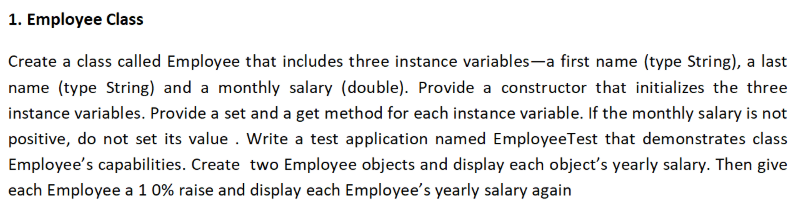
\includegraphics[width=0.8\textwidth]{./Assets/Task requirements/Assignment7/1.png}
    \caption{Problem 1 Task Requirement}
\end{figure}

\begin{lstlisting}[language=Java, caption=Employee and EmployeeTest Classes]
public class Employee {
    private String firstName;
    private String lastname;
    private double monthySalary;

    public Employee(String firstName, String lastname, double monthySalary) {
        this.firstName = firstName;
        this.lastname = lastname;
        if (monthySalary >= 0) {
            this.monthySalary = monthySalary;
        } else {
            this.monthySalary = 0.0;
        }
    }

    public String getFirstName() {
        return firstName;
    }
    public String getLastName() {
        return lastname;
    }
    public double getMonthySalary() {
        return monthySalary;
    }
    public void setFirstName(String firstName) {
        this.firstName = firstName;
    }
    public void setLastname(String lastname) {
        this.lastname = lastname;
    }
    public void setMonthySalary(double monthySalary) {
        if (monthySalary >= 0) {
            this.monthySalary = monthySalary;
        }
    }
    public double getYearlySalary() {
        // yearly bonus
        return monthySalary * 13;
    }
    public void giveRaise(double raisePercentage) {
        this.monthySalary += monthySalary * raisePercentage / 100;
    }
}

public class EmployeeTest {
    public static void main(String[] args) {
        Employee emp1101 = new Employee("Nguyen", "A", 90);
        Employee emp1100 = new Employee("Dao", "B", 1000);

        System.out.println("Salary of " + emp1101.getFirstName() + " " + emp1101.getLastName() + ": " + emp1101.getMonthySalary());
        System.out.println("Salary of " + emp1100.getFirstName() + " " + emp1100.getLastName() + ": " + emp1100.getMonthySalary());

        // give each employee a 10% raise
        emp1101.giveRaise(10);
        emp1100.giveRaise(10);

        emp1100.setMonthySalary(-90);
        emp1100.setFirstName("Tien");
        emp1101.setLastname("T");

        System.out.println("Salary of " + emp1101.getFirstName() + " " + emp1101.getLastName() + " after 10% raise: " + emp1101.getMonthySalary());
        System.out.println("Salary of " + emp1100.getFirstName() + " " + emp1100.getLastName() + " after 10% raise: " + emp1100.getMonthySalary());

        // display yearly salary after the raise
        System.out.println("Yearly salary of " + emp1101.getFirstName() + " " + emp1101.getLastName() + " after 10% raise: " + emp1101.getYearlySalary());
        System.out.println("Yearly salary of " + emp1100.getFirstName() + " " + emp1100.getLastName() + " after 10% raise: " + emp1100.getYearlySalary());
    }
}
\end{lstlisting}

\subsection*{3. Modify the CellPhone Project}

\begin{figure}[H]
    \centering

    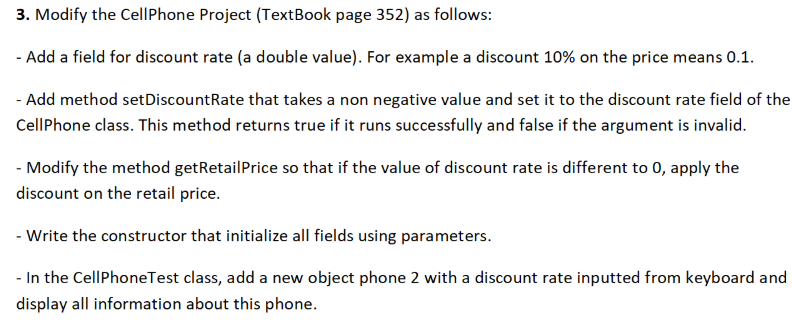
\includegraphics[width=0.8\textwidth]{./Assets/Task requirements/Assignment7/3.png}
    \caption{Problem 3 Task Requirement}
\end{figure}

\begin{lstlisting}[language=Java, caption=CellPhone and CellPhoneTest Classes]
/**
 * The CellPhone class holds data about a cell phone.
 */

public class CellPhone {

    // Fields
    private String manufact; // Manufacturer
    private String model;    // Model
    private double retailPrice; // Retail price

    private double discountRate;

    /**
     * Constructor
     * @param man The phone's manufacturer.
     * @param mod The phone's model number.
     * @param price The phone's retail price.
     */
    public CellPhone(String man, String mod, double price) {
        manufact = man;
        model = mod;
        retailPrice = price;
    }

    public CellPhone(String man, String mod, double price, double discount) {
        manufact = man;
        model = mod;
        retailPrice = price;
        discountRate = discount;
    }

    /**
     * The setManufact method sets the phone's manufacturer name.
     * @param man The phone's manufacturer.
     */
    public void setManufact(String man) {
        manufact = man;
    }

    /**
     * The setModel method sets the phone's model number.
     * @param mod The phone's model number.
     */
    public void setModel(String mod) {
        model = mod;
    }

    /**
     * The setRetailPrice method sets the phone's retail price.
     * @param price The phone's retail price.
     */
    public void setRetailPrice(double price) {
        retailPrice = price;
    }

    /**
     * getManufact method
     * @return The name of the phone's manufacturer.
     */
    public String getManufact() {
        return manufact;
    }

    /**
     * getModel method
     * @return The phone's model number.
     */
    public String getModel() {
        return model;
    }

    /**
     * getRetailPrice method
     * @return The phone's retail price.
     */
    public double getRetailPrice() {
        if (discountRate > 0){
            retailPrice -= retailPrice * discountRate;
        }
        return retailPrice;
    }

    public boolean setDiscountRate(double d) {
        if(d > 0 && d < 1) {
            this.discountRate = d;
            return true;
        }
        System.out.println("Invalid discount rate");
        return false;
    }

    public double getDiscountRate() {
        return discountRate;
    }
}

import java.util.Scanner;

/**
 * This program runs a simple test of the CellPhone class.
 */
public class CellPhoneTest {

    public static void main(String[] args) {
        String testMan; // To hold a manufacturer
        String testMod; // To hold a model number
        double testPrice; // To hold a price
        double discount;

        // Create a Scanner object for keyboard input.
        Scanner keyboard = new Scanner(System.in);

        // Get the manufacturer name.
        System.out.print("Enter the manufacturer: ");
        testMan = keyboard.nextLine();

        // Get the model number.
        System.out.print("Enter the model number: ");
        testMod = keyboard.nextLine();

        // Get the retail price.
        System.out.print("Enter the retail price: ");
        testPrice = keyboard.nextDouble();

        // Create an instance of the CellPhone class,
        // passing the data that was entered as arguments
        // to the constructor.
        CellPhone phone = new CellPhone(testMan, testMod, testPrice);
        CellPhone phone2 = new CellPhone("Apple", "Iphone 20", 9000);

        // Get the data from the phone and display it.
        System.out.println();
        System.out.println("Here is the data that you provided:");
        System.out.println("Manufacturer: " + phone.getManufact());
        System.out.println("Model number: " + phone.getModel());
        System.out.println("Retail price: " + phone.getRetailPrice());

        System.out.println();
        System.out.print("Enter the discount for phone 2: ");
        discount = keyboard.nextDouble();
        phone2.setDiscountRate(discount);

        System.out.println();
        System.out.println("Here is the data that you provided:");
        System.out.println("Manufacturer: " + phone2.getManufact());
        System.out.println("Model number: " + phone2.getModel());
        System.out.println("Discount rate: " + phone2.getDiscountRate());
        System.out.println("Retail price: " + phone2.getRetailPrice());

        keyboard.close();
    }
}
\end{lstlisting}

\subsection*{6.5}

\begin{figure}[H]
    \centering
    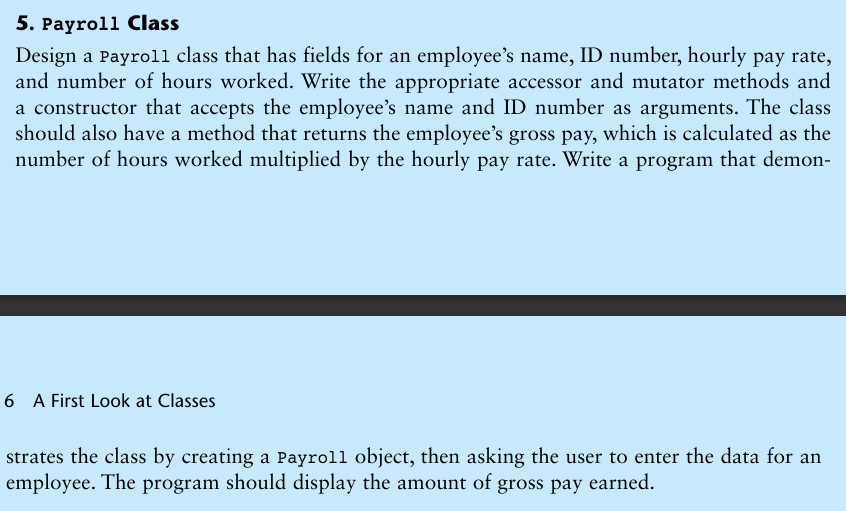
\includegraphics[width=0.8\textwidth]{./Assets/Task requirements/Assignment7/6.5.png}
    \caption{6.5 Task Requirement}
\end{figure}

\begin{lstlisting}[language=Java, caption=payRoll and payRollTest Classes]
public class payRoll {
    private String employeeName;
    private String id;
    private double hourlyRate = 0.0;
    private int hourWorked = 0;

    payRoll(String employeeName, String id) {
        this.employeeName = employeeName;
        this.id = id;
    }

    public String getName() {
        return employeeName;
    }

    public String getId() {
        return id;
    }

    public double getHourlyRate() {
        return hourlyRate;
    }

    public int getHourWorked() {
        return hourWorked;
    }

    public double getGrossPay() {
        return hourlyRate * hourWorked;
    }

    public void setEmployeeName(String employeeName) {
        this.employeeName = employeeName;
    }

    public void setId(String id) {
        this.id = id;
    }

    public void setHourlyRate(double hourlyRate) {
        if (hourlyRate > 0) {
            this.hourlyRate = hourlyRate;
        }
    }

    public void setHourWorked(int hourWorked) {
        if (hourWorked > 0) {
            this.hourWorked = hourWorked;
        }
    }
}

import java.util.Scanner;

public class payRollTest {
    public static void main(String[] args) {

        payRoll PRex = new payRoll("test", "0000");

        Scanner sc = new Scanner(System.in);

        System.out.println();
        System.out.println("Please enter the information for a new employee: ");
        System.out.print("Name: ");
        PRex.setEmployeeName(sc.nextLine());

        System.out.print("Employee id: ");
        PRex.setId(sc.nextLine());

        System.out.print("Employee's hourly rate: ");
        PRex.setHourlyRate(sc.nextDouble());

        System.out.print("How many hours have they worked? ");
        PRex.setHourWorked(sc.nextInt());

        System.out.println("Employee " + PRex.getName() + " gross pay: " + PRex.getGrossPay());

        sc.close();
    }
}
\end{lstlisting}

\subsection*{6.6}

\begin{figure}[H]
    \centering
    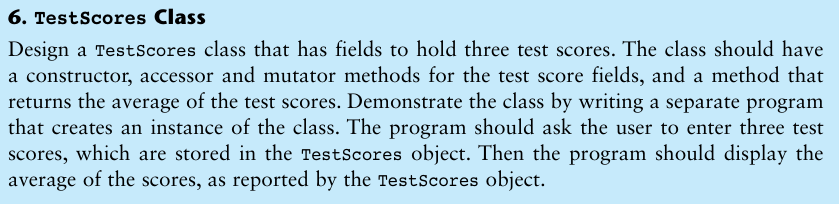
\includegraphics[width=0.8\textwidth]{./Assets/Task requirements/Assignment7/6.6.png}
    \caption{6.6 Task Requirement}
\end{figure}

\begin{lstlisting}[language=Java, caption=Main and TestScore Classes]
import java.util.Scanner;

public class Main {
    public static void main(String[] args) {
        double CS310Score;
        double CS365Score;
        double CS360Score;
        Scanner sc = new Scanner(System.in);

        TestScore TrungTS = new TestScore(10, 10, 10);
        System.out.println(TrungTS.getAverageScore());

        System.out.print("Enter the first subject score: ");
        CS310Score = sc.nextDouble();

        System.out.print("Enter the second subject score: ");
        CS365Score = sc.nextDouble();

        System.out.print("Enter the third subject score: ");
        CS360Score = sc.nextDouble();

        TestScore Fall2024TrungTS = new TestScore(CS310Score, CS365Score, CS360Score);
        System.out.println("Your Fall 2024 average tests score: " + Fall2024TrungTS.getAverageScore());

        sc.close();
    }
}

public class TestScore {
    private double testScore1;
    private double testScore2;
    private double testScore3;

    TestScore(double testScore1, double testScore2, double testScore3) {
        if ((testScore1 >= 0 && testScore2 >= 0 && testScore3 >= 0) &&
            (testScore1 <= 10 && testScore2 <= 10 && testScore3 <= 10)) {
            this.testScore1 = testScore1;
            this.testScore2 = testScore2;
            this.testScore3 = testScore3;
        }
    }

    public double getTestScore1() {
        return testScore1;
    }

    public double getTestScore2() {
        return testScore2;
    }

    public double getTestScore3() {
        return testScore3;
    }

    public void setTestScore1(double testScore1) {
        if (testScore1 >= 0 && testScore1 <= 10) {
            this.testScore1 = testScore1;
        }
    }

    public void setTestScore2(double testScore2) {
        if (testScore2 >= 0 && testScore2 <= 10) {
            this.testScore2 = testScore2;
        }
    }

    public void setTestScore3(double testScore3) {
        if (testScore3 >= 0 && testScore3 <= 10) {
            this.testScore3 = testScore3;
        }
    }

    public double getAverageScore() {
        return (this.testScore1 + this.testScore2 + this.testScore3) / 3;
    }
}
\end{lstlisting}

\subsection*{6.8}

\begin{figure}[H]
    \centering
    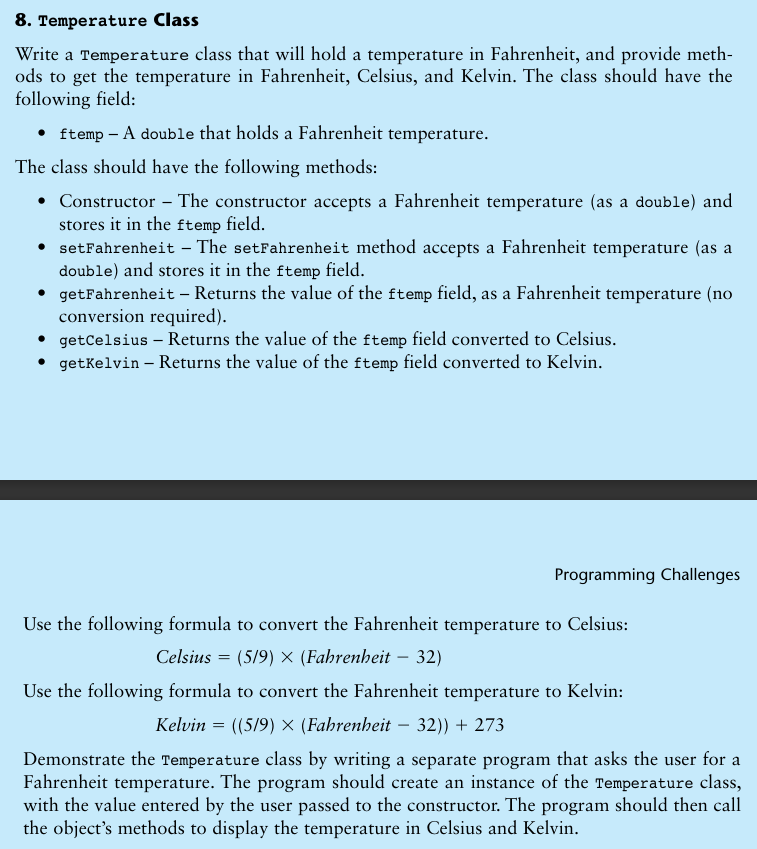
\includegraphics[width=0.8\textwidth]{./Assets/Task requirements/Assignment7/6.8.png}
    \caption{6.8 Task Requirement}
\end{figure}

\begin{lstlisting}[language=Java, caption=Temperature Class]
import java.util.Scanner;

public class Temperature {
    private double ftemp;

    Temperature(double ftemp) {
        this.ftemp = ftemp;
    }

    public double getFahrenheit() {
        return ftemp;
    }

    public double getCelsius() {
        return (5.0 / 9) * (ftemp - 32);
    }

    public double getKelvin() {
        return ((5.0 / 9) * (ftemp - 32)) + 273;
    }

    public void setFahrenheit(double Fahrenheit) {
        this.ftemp = Fahrenheit;
    }

    public static void main(String[] args) {
        Scanner sc = new Scanner(System.in);

        System.out.print("Enter a temperature in Fahrenheit: ");
        double ftemp = sc.nextDouble();

        Temperature temp = new Temperature(ftemp);

        System.out.println("Temperature in Fahrenheit: " + temp.getFahrenheit());
        System.out.printf("Temperature in Celsius: %.2f\n", temp.getCelsius());
        System.out.printf("Temperature in Kelvin: %.2f\n", temp.getKelvin());

        sc.close();
    }
}
\end{lstlisting}

\section*{Assignment 8}

\textbf{Contributor}: Nguyen Quang Huy - 1677664

\subsection*{7.1}

\begin{figure}[H]
    \centering
    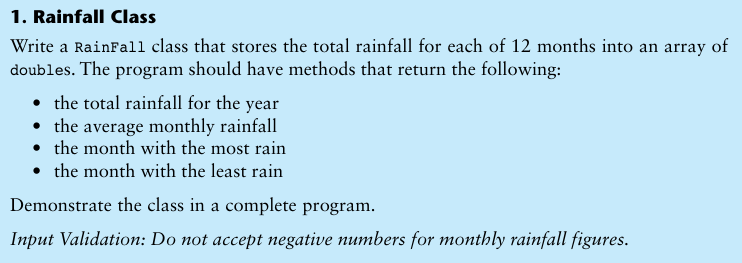
\includegraphics[width=0.8\textwidth]{./Assets/Task requirements/Assignment8/7.1.png}
    \caption{7.1 Task Requirement}
\end{figure}

\begin{lstlisting}[language=Java, caption=Rainfall.java]
// Rainfall.java
public class Rainfall {
    private double[] monthlyRainfall;

    // Constructor with input validation
    public Rainfall(double[] rainfall) {
        monthlyRainfall = new double[12];
        for (int i = 0; i < 12; i++) {
            if (rainfall[i] < 0) {
                throw new IllegalArgumentException("Rainfall figures cannot be negative.");
            }
            monthlyRainfall[i] = rainfall[i];
        }
    }

    // Calculate total rainfall
    public double getTotalRainfall() {
        double total = 0;
        for (double rain : monthlyRainfall) {
            total += rain;
        }
        return total;
    }

    // Calculate average monthly rainfall
    public double getAverageRainfall() {
        return getTotalRainfall() / monthlyRainfall.length;
    }

    // Find the month with the most rain
    public int getMonthWithMostRain() {
        int month = 0;
        double maxRain = monthlyRainfall[0];
        for (int i = 1; i < monthlyRainfall.length; i++) {
            if (monthlyRainfall[i] > maxRain) {
                maxRain = monthlyRainfall[i];
                month = i;
            }
        }
        return month + 1; // Return month (1-12)
    }

    // Find the month with the least rain
    public int getMonthWithLeastRain() {
        int month = 0;
        double minRain = monthlyRainfall[0];
        for (int i = 1; i < monthlyRainfall.length; i++) {
            if (monthlyRainfall[i] < minRain) {
                minRain = monthlyRainfall[i];
                month = i;
            }
        }
        return month + 1; // Return month (1-12)
    }
}
\end{lstlisting}

\begin{lstlisting}[language=Java, caption=RainFallDemo.java]
// RainfallDemo.java
import java.util.Scanner;

public class RainfallDemo {
    public static void main(String[] args) {
        Scanner input = new Scanner(System.in);
        double[] rainfall = new double[12];

        System.out.println("Enter the total rainfall for each month:");

        // Input rainfall data with validation
        for (int i = 0; i < 12; i++) {
            while (true) {
                System.out.print("Month " + (i + 1) + ": ");
                rainfall[i] = input.nextDouble();
                if (rainfall[i] < 0) {
                    System.out.println("Rainfall cannot be negative. Please enter a valid number.");
                } else {
                    break;
                }
            }
        }

        // Create Rainfall object and call methods
        Rainfall rainData = new Rainfall(rainfall);

        // Display results
        System.out.printf("Total Rainfall: %.2f\n", rainData.getTotalRainfall());
        System.out.printf("Average Monthly Rainfall: %.2f\n", rainData.getAverageRainfall());
        System.out.println("Month with Most Rain: " + rainData.getMonthWithMostRain());
        System.out.println("Month with Least Rain: " + rainData.getMonthWithLeastRain());

        input.close();
    }
}
\end{lstlisting}

\subsection*{7.2}

\begin{figure}[H]
    \centering
    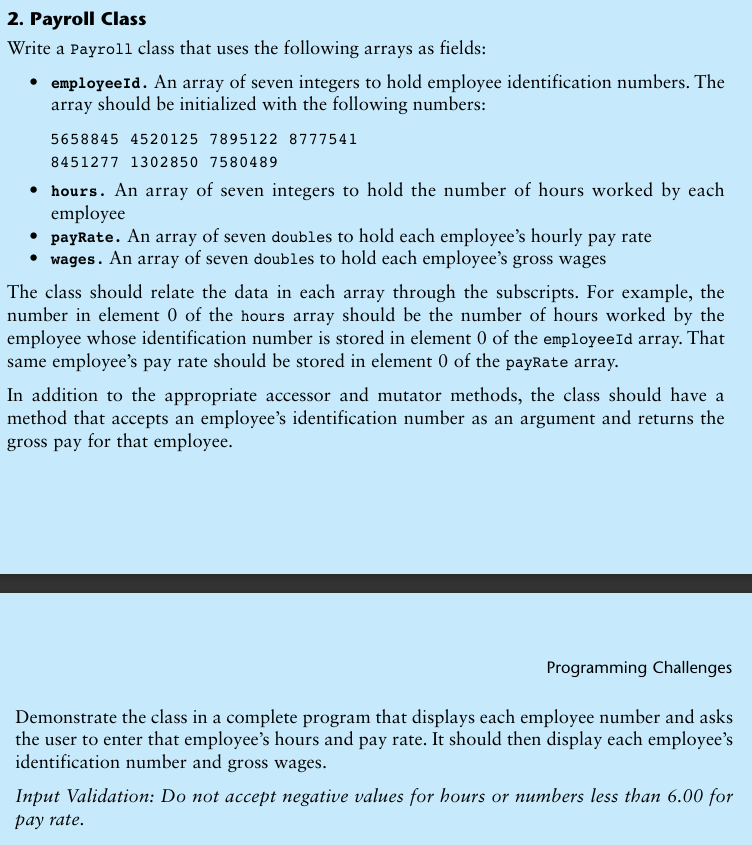
\includegraphics[width=0.8\textwidth]{./Assets/Task requirements/Assignment8/7.2.png}
    \caption{7.2 Task Requirement}
\end{figure}

\begin{lstlisting}[language=Java, caption=Payroll.java]
// Payroll.java
public class Payroll {
    // Declare arrays for fields
    private int[] employeeId = { 5658845, 4520125, 7895122, 8777541, 8451277, 1302850, 7580489 };
    private int[] hours = new int[7];       // Hours worked by each employee
    private double[] payRate = new double[7]; // Hourly pay rate
    private double[] wages = new double[7];   // Total wages for each employee

    // Set hours worked with input validation
    public void setHours(int index, int hoursWorked) {
        if (hoursWorked < 0) {
            throw new IllegalArgumentException("Hours cannot be negative.");
        }
        hours[index] = hoursWorked;
    }

    // Set pay rate with input validation
    public void setPayRate(int index, double rate) {
        if (rate < 6.00) {
            throw new IllegalArgumentException("Pay rate must be at least 6.00.");
        }
        payRate[index] = rate;
    }

    // Calculate wages for each employee
    public void calculateWages() {
        for (int i = 0; i < employeeId.length; i++) {
            wages[i] = hours[i] * payRate[i];
        }
    }

    // Return employee ID
    public int getEmployeeId(int index) {
        return employeeId[index];
    }

    // Return total wages for an employee
    public double getWages(int index) {
        return wages[index];
    }
}
\end{lstlisting}

\begin{lstlisting}[language=Java, caption=PayrollDemo.java]
// PayrollDemo.java
import java.util.Scanner;

public class PayrollDemo {
    public static void main(String[] args) {
        Scanner input = new Scanner(System.in);
        Payroll payroll = new Payroll();

        System.out.println("Enter hours worked and pay rate for each employee:");

        // Loop to input data for each employee
        for (int i = 0; i < 7; i++) {
            int hoursWorked;
            double payRate;

            // Display employee ID
            System.out.println("Employee ID: " + payroll.getEmployeeId(i));

            // Input hours worked with validation
            while (true) {
                System.out.print("Enter hours worked: ");
                hoursWorked = input.nextInt();
                if (hoursWorked >= 0) {
                    break;
                }
                System.out.println("Hours cannot be negative. Please try again.");
            }
            payroll.setHours(i, hoursWorked);

            // Input hourly pay rate with validation
            while (true) {
                System.out.print("Enter hourly pay rate: ");
                payRate = input.nextDouble();
                if (payRate >= 6.00) {
                    break;
                }
                System.out.println("Pay rate must be at least 6.00. Please try again.");
            }
            payroll.setPayRate(i, payRate);
        }

        // Calculate wages
        payroll.calculateWages();

        // Display results
        System.out.println("\nEmployee Wages:");
        for (int i = 0; i < 7; i++) {
            System.out.printf("Employee ID: %d | Gross Wages: %.2f\n",
                              payroll.getEmployeeId(i), payroll.getWages(i));
        }

        input.close();
    }
}
\end{lstlisting}

\subsection*{7.3}

\begin{figure}[H]
    \centering
    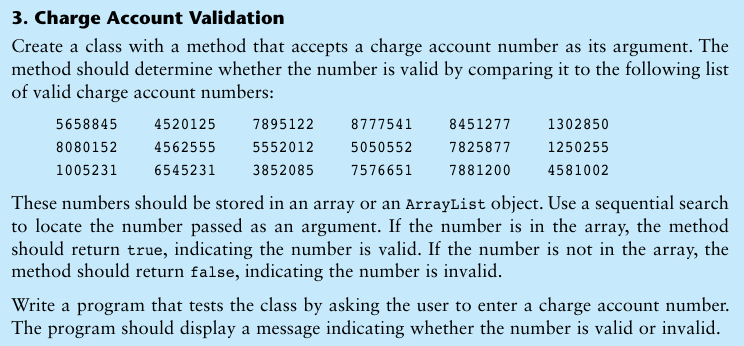
\includegraphics[width=0.8\textwidth]{./Assets/Task requirements/Assignment8/7.3.png}
    \caption{7.3 Task Requirement}
\end{figure}

\begin{lstlisting}[language=Java,caption=ChargeAccount.java]
public class ChargeAccount {
    private int[] validAccountNumbers = {
        5658845, 4520125, 7895122, 8777541, 8451277, 1302850,
        8080152, 4562555, 5552012, 5050552, 7825877, 1250255,
        1005231, 6545231, 3852085, 7576651, 7881200, 4581002
    };


    public boolean isValidAccount(int accountNumber) {
        for (int validNumber : validAccountNumbers) {
            if (validNumber == accountNumber) {
                return true;
            }
        }
        return false;
    }
}
\end{lstlisting}

\begin{lstlisting}[language=Java, caption=ChargeAccountDemo.java]
import java.util.Scanner;

public class ChargeAccountDemo {
    public static void main(String[] args) {
        Scanner input = new Scanner(System.in);
        ChargeAccount accountValidator = new ChargeAccount();


        System.out.print("Enter a charge account number to validate: ");
        int accountNumber = input.nextInt();

        if (accountValidator.isValidAccount(accountNumber)) {
            System.out.println("The account number " + accountNumber + " is VALID.");
        } else {
            System.out.println("The account number " + accountNumber + " is INVALID.");
        }

        input.close();
    }
}
\end{lstlisting}

\subsection*{2. Circle class}

\begin{figure}[H]
    \centering
    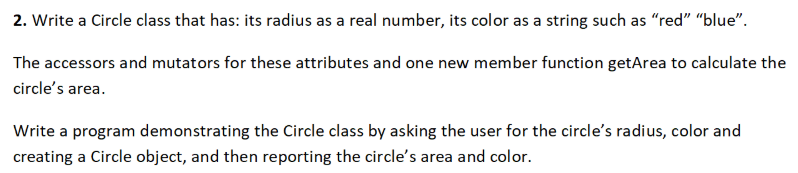
\includegraphics[width=0.8\textwidth]{./Assets/Task requirements/Assignment8/2.png}
    \caption{Problem 2 Task Requirement}
\end{figure}

\begin{lstlisting}[language=Java, caption=Circle.java]
public class Circle {

    private double radius;
    private String color;

    public Circle(double radius, String color) {
        this.radius = radius;
        this.color = color;
    }

    public double getRadius() {
        return radius;
    }

    public String getColor() {
        return color;
    }

    public void setRadius(double radius) {
        this.radius = radius;
    }

    public void setColor(String color) {
        this.color = color;
    }

    public double getArea() {
        return Math.PI * Math.pow(radius, 2);
    }
}
\end{lstlisting}

\begin{lstlisting}[language=Java, caption=CircleTest.java]
import java.util.Scanner;

public class CircleTest {
    public static void main(String[] args) {

        Scanner scanner = new Scanner(System.in);

        System.out.print("Enter radius: ");
        double radius = scanner.nextDouble();
        scanner.nextLine();

        String color = "";
        boolean validColor = false;
        while (!validColor) {
            System.out.print("Enter color (red or blue): ");
            color = scanner.nextLine().toLowerCase();
            if (color.equals("red") || color.equals("blue")) {
                validColor = true;
            } else {
                System.out.println("Invalid color. Please enter 'red' or 'blue'.");
            }
        }

        Circle circle = new Circle(radius, color);

        System.out.printf("The area is: %.2f\n", circle.getArea());
        System.out.println("The color is: " + circle.getColor());

        scanner.close();
    }
}
\end{lstlisting}

\subsection*{3. Employee class}

\begin{figure}[H]
    \centering
    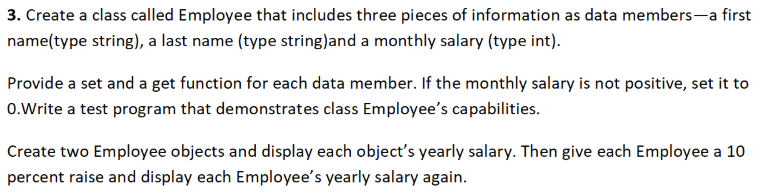
\includegraphics[width=0.8\textwidth]{./Assets/Task requirements/Assignment8/3.png}
    \caption{Problem 3 Requirement}
\end{figure}

\begin{lstlisting}[language=Java, caption=Employee.java]
public class Employee {

    private String firstName;
    private String lastName;
    private int monthlySalary;

    public Employee(String firstName, String lastName, int monthlySalary) {
        this.firstName = firstName;
        this.lastName = lastName;
        this.monthlySalary = monthlySalary;
    }

    public String getFirstName() {
        return firstName;
    }

    public void setFirstName(String firstName) {
        this.firstName = firstName;
    }

    public String getLastName() {
        return lastName;
    }

    public void setLastName(String lastName) {
        this.lastName = lastName;
    }

    public int getMonthlySalary() {
        return monthlySalary;
    }

    public void setMonthlySalary(int monthlySalary) {
        if (monthlySalary > 0) {
            this.monthlySalary = monthlySalary;
        } else {
            this.monthlySalary = 0;
        }
    }

    public int getYearlySalary() {
        return monthlySalary * 12;
    }

    public void applyRaise() {
        monthlySalary += monthlySalary * 0.10;
    }
}
\end{lstlisting}

\begin{lstlisting}[language=Java, caption=EmployeeTest.java]
public class EmployeeTest {
    public static void main(String[] args) {
        Employee employee1 = new Employee("Quang", "Huy", 3000);
        Employee employee2 = new Employee("Naruto", "Sasuke", 2500);

        System.out.println(employee1.getFirstName() + " " + employee1.getLastName() +
            "'s yearly salary: " + employee1.getYearlySalary());
        System.out.println(employee2.getFirstName() + " " + employee2.getLastName() +
            "'s yearly salary: " + employee2.getYearlySalary());

        employee1.applyRaise();
        employee2.applyRaise();

        System.out.println("After 10% raise:");
        System.out.println(employee1.getFirstName() + " " + employee1.getLastName() +
            "'s yearly salary: " + employee1.getYearlySalary());
        System.out.println(employee2.getFirstName() + " " + employee2.getLastName() +
            "'s yearly salary: " + employee2.getYearlySalary());
    }
}
\end{lstlisting}

\subsection*{4. Account class}

\begin{figure}[H]
    \centering
    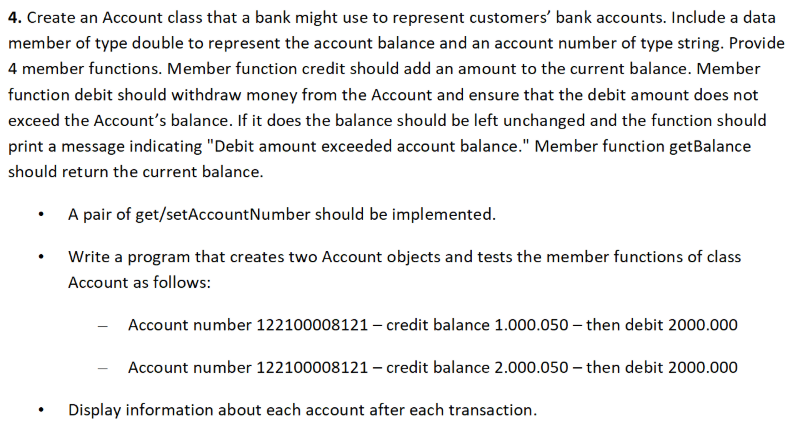
\includegraphics[width=0.8\textwidth]{./Assets/Task requirements/Assignment8/4.png}
    \caption{Problem 4 Requirement}
\end{figure}

\begin{lstlisting}[language=Java, caption=Account.java]
public class Account {
    private double balance;
    private String accountNumber;

    public Account(String accNumber, double initialBalance) {
        accountNumber = accNumber;
        balance = initialBalance;
    }

    public void credit(double amount) {
        balance += amount;
    }

    public void debit(double amount) {
        if (amount > balance) {
            System.out.println("Debit amount exceeded account balance.");
        } else {
            balance -= amount;
        }
    }

    public double getBalance() {
        return balance;
    }

    public String getAccountNumber() {
        return accountNumber;
    }

    public void setAccountNumber(String accNumber) {
        accountNumber = accNumber;
    }

    public void displayAccountInfo() {
        System.out.println("Account number: " + accountNumber);
        System.out.println("Balance: " + balance);
    }
}
\end{lstlisting}

\begin{lstlisting}[language=Java, caption=ATM.java]
public class ATM {
    public static void main(String[] args) {
        Account account1 = new Account("122100008121", 1000050);
        Account account2 = new Account("122100008121", 2000050);

        System.out.println("Before transactions:");
        account1.displayAccountInfo();
        account2.displayAccountInfo();

        account1.credit(1000050);
        account1.debit(2000000);

        account2.credit(2000050);
        account2.debit(2000000);

        System.out.println("After transaction:");
        account1.displayAccountInfo();
        account2.displayAccountInfo();
    }
}
\end{lstlisting}

\section*{Assignment 10}

\textbf{Contributor}: Nguyen Duy Khoi - 1677395

\subsection*{1. Complex class}

\begin{figure}[H]
    \centering
    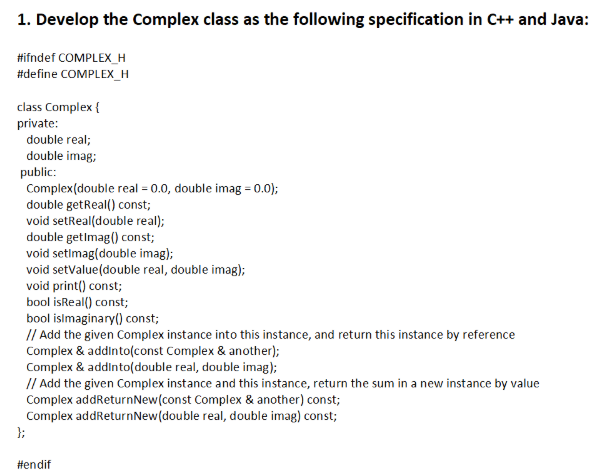
\includegraphics[width=0.8\textwidth]{./Assets/Task requirements/Assignment10/1.png}
    \caption{Problem 1}
\end{figure}

\subsubsection*{1. C++}
\begin{lstlisting}[language=C++, caption=Complex.cpp]
#include "Complex.h"
#include <iostream>

using namespace std;

Complex::Complex(double real, double imag) : real(real), imag(imag) {}

double Complex::getReal() const {
    return real;
}

void Complex::setReal(double real) {
    this->real = real;
}

double Complex::getImag() const {
    return imag;
}

void Complex::setImag(double imag) {
    this->imag = imag;
}

void Complex::setValue(double real, double imag) {
    this->real = real;
    this->imag = imag;
}

void Complex::print() const {
    cout << real;
    if (imag >= 0) {
        cout << " + " << imag << "i" << endl;
    } else {
        cout << " - " << -imag << "i" << endl;
    }
}

bool Complex::isReal() const {
    return imag == 0.0;
}

bool Complex::isImaginary() const {
    return real == 0.0;
}

Complex & Complex::addInto(const Complex & another) {
    this->real += another.real;
    this->imag += another.imag;
    return *this;
}

Complex & Complex::addInto(double real, double imag) {
    this->real += real;
    this->imag += imag;
    return *this;
}

Complex Complex::addReturnNew(const Complex & another) const {
    return Complex(this->real + another.real, this->imag + another.imag);
}

Complex Complex::addReturnNew(double real, double imag) const {
    return Complex(this->real + real, this->imag + imag);
}
\end{lstlisting}

\begin{lstlisting}[language=C++, caption=Complex.h]
#ifndef COMPLEX_H
#define COMPLEX_H

class Complex {
private:
    double real;
    double imag;

public:
    Complex(double real = 0.0, double imag = 0.0);

    double getReal() const;
    void setReal(double real);

    double getImag() const;
    void setImag(double imag);

    void setValue(double real, double imag);

    void print() const;

    bool isReal() const;
    bool isImaginary() const;

    Complex & addInto(const Complex & another);
    Complex & addInto(double real, double imag);

    Complex addReturnNew(const Complex & another) const;
    Complex addReturnNew(double real, double imag) const;
};

#endif
\end{lstlisting}

\begin{lstlisting}[language=C++, caption=Main.cpp]
#include <iostream>
#include "Complex.h"

int main() {
    Complex c1(2.0, 3.0);
    Complex c2(1.0, 4.0);
    Complex c3 = c1.addReturnNew(c2);
    c1.print();
    c2.print();
    c3.print();

    c1.addInto(c2);
    c1.print();

    return 0;
}
\end{lstlisting}

\subsubsection*{1. Java}
\begin{lstlisting}[language=Java, caption=Complex.java]
public class Complex {
    private double real;
    private double imag;

    public Complex(double real, double imag) {
        this.real = real;
        this.imag = imag;
    }

    public Complex() {
        this(0.0, 0.0);
    }

    public double getReal() {
        return real;
    }

    public void setReal(double real) {
        this.real = real;
    }

    public double getImag() {
        return imag;
    }

    public void setImag(double imag) {
        this.imag = imag;
    }

    public void setValue(double real, double imag) {
        this.real = real;
        this.imag = imag;
    }

    public void print() {
        System.out.print(real);
        if (imag >= 0) {
            System.out.println(" + " + imag + "i");
        } else {
            System.out.println(" - " + -imag + "i");
        }
    }

    public boolean isReal() {
        return imag == 0.0;
    }

    public boolean isImaginary() {
        return real == 0.0;
    }

    public Complex addInto(Complex another) {
        this.real += another.real;
        this.imag += another.imag;
        return this;
    }

    public Complex addInto(double real, double imag) {
        this.real += real;
        this.imag += imag;
        return this;
    }

    public Complex addReturnNew(Complex another) {
        return new Complex(this.real + another.real, this.imag + another.imag);
    }

    public Complex addReturnNew(double real, double imag) {
        return new Complex(this.real + real, this.imag + imag);
    }
}
\end{lstlisting}

\begin{lstlisting}[language=Java, caption=TestComplex.java]
public class TestComplex {
    public static void main(String[] args) {

        Complex c1 = new Complex(2.0, 3.0);
        Complex c2 = new Complex(1.0, 4.0);
        Complex c3 = c1.addReturnNew(c2);
        c1.print();
        c2.print();
        c3.print();

        c1.addInto(c2);
        c1.print();
    }
}
\end{lstlisting}

\subsection*{2. Date class}
\begin{figure}[H]
    \centering
    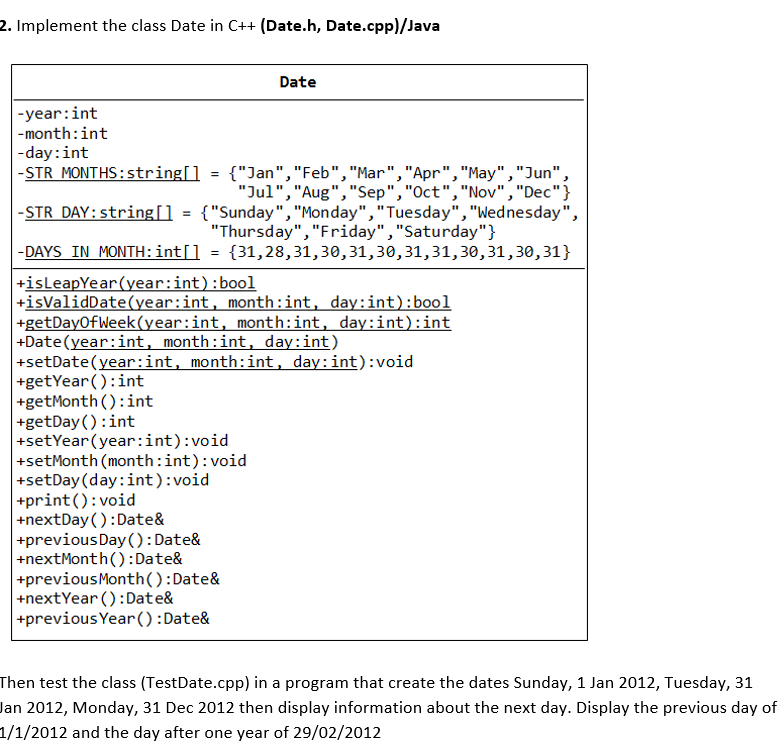
\includegraphics[width=0.8\textwidth]{./Assets/Task requirements/Assignment10/2.png}
    \caption{Problem 2}
\end{figure}

\subsubsection*{2. C++}

\begin{lstlisting}[language=C++, caption=Date.cpp]
#include "Date.h"
#include <iostream>
#include <string>

Date::Date(int day, int month, int year) : day(day), month(month), year(year) {}

int Date::getDay() const {
    return day;
}

int Date::getMonth() const {
    return month;
}

int Date::getYear() const {
    return year;
}

void Date::setDay(int day) {
    this->day = day;
}

void Date::setMonth(int month) {
    this->month = month;
}

void Date::setYear(int year) {
    this->year = year;
}

bool Date::isValid() const {
    if (month < 1 || month > 12 || day < 1 || day > 31) {
        return false;
    }

    if (month == 2) {
        if ((year % 4 == 0 && year % 100 != 0) || (year % 400 == 0)) {
        }
        return day <= 28;
    }

    if (month == 4 || month == 6 || month == 9 || month == 11) {
        return day <= 30;
    }

    return true;
}

std::string Date::toString() const {
    return std::to_string(day) + "/" + std::to_string(month) + "/" + std::to_string(year);
}
\end{lstlisting}

\begin{lstlisting}[language=C++, caption=Date.h]
#ifndef DATE_H
#define DATE_H
#include <string>

class Date {
private:
    int day;
    int month;
    int year;

public:
    Date(int day, int month, int year);

    int getDay() const;
    int getMonth() const;
    int getYear() const;

    void setDay(int day);
    void setMonth(int month);
    void setYear(int year);

    bool isValid() const;

    std::string toString() const;
};

#endif
\end{lstlisting}

\begin{lstlisting}[language=C++, caption=DateFunctions.cpp]
#include <iostream>
#include "Date.h"

Date getNextDay(const Date &d) {
    int day = d.getDay();
    int month = d.getMonth();
    int year = d.getYear();

    day++;
    Date temp(day, month, year);

    if (!temp.isValid()) {
        day = 1;
        month++;
        temp.setDay(day);
        temp.setMonth(month);

        if (!temp.isValid()) {
            month = 1;
            year++;
            temp.setMonth(month);
            temp.setYear(year);
        }
    }
    return temp;
}

Date getPreviousDay(const Date &d) {
    int day = d.getDay();
    int month = d.getMonth();
    int year = d.getYear();

    day--;
    Date temp(day, month, year);

    if (!temp.isValid()) {
        month--;
        if (month < 1) {
            month = 12;
            year--;
        }

        temp.setMonth(month);
        temp.setYear(year);
        if (month == 2) {
            temp.setDay((year % 4 == 0 && year % 100 != 0) || (year % 400 == 0) ? 29 : 28);
        } else if (month == 4 || month == 6 || month == 9 || month == 11) {
            temp.setDay(30);
        } else {
            temp.setDay(31);
        }
    }
    return temp;
}

Date getDateAfterOneYear(const Date &d) {
    int day = d.getDay();
    int month = d.getMonth();
    int year = d.getYear();

    year++;
    Date temp(day, month, year);

    if (!temp.isValid()) {
        if (month == 2 && day == 29 && !(year % 4 == 0 && year % 100 != 0) && !(year % 400 == 0)) {
            temp.setDay(28);
        }
    }
    return temp;
}
\end{lstlisting}

\begin{lstlisting}[language=C++, caption=main.cpp]
#include <iostream>
#include "Date.h"

int main() {
    Date date1(1, 1, 2012);
    Date date2(31, 1, 2012);
    Date date3(31, 12, 2012);

    std::cout << "Current Date: " << date1.toString() << " | Next Day: " << getNextDay(date1).toString() << std::endl;
    std::cout << "Current Date: " << date2.toString() << " | Next Day: " << getNextDay(date2).toString() << std::endl;
    std::cout << "Current Date: " << date3.toString() << " | Next Day: " << getNextDay(date3).toString() << std::endl;

    Date prevDay = getPreviousDay(date1);
    std::cout << "Previous Day of 1/1/2012: " << prevDay.toString() << std::endl;

    Date leapYearDate(29, 2, 2012);
    Date nextYearDate = getDateAfterOneYear(leapYearDate);
    std::cout << "One year after 29/2/2012: " << nextYearDate.toString() << std::endl;

    return 0;
}
\end{lstlisting}

\subsubsection*{2. Java}

\begin{lstlisting}[language=Java, caption=Date.java]
public class Date {
    private int day;
    private int month;
    private int year;

    // Constructor
    public Date(int day, int month, int year) {
        this.day = day;
        this.month = month;
        this.year = year;
    }

    // Getters
    public int getDay() { return day; }
    public int getMonth() { return month; }
    public int getYear() { return year; }

    // Setters
    public void setDay(int day) { this.day = day; }
    public void setMonth(int month) { this.month = month; }
    public void setYear(int year) { this.year = year; }

    // Display method
    public void display() {
        System.out.println(day + "/" + month + "/" + year);
    }

    // Convert to String
    public String toString() {
        return day + "/" + month + "/" + year;
    }

    // Validation method
    public boolean isValid() {
        if (month < 1 || month > 12 || day < 1 || day > 31) {
            return false;
        }
        if (month == 2) {
            if ((year % 4 == 0 && year % 100 != 0) || (year % 400 == 0)) {
                return day <= 29;
            }
            return day <= 28;
        }
        if (month == 4 || month == 6 || month == 9 || month == 11) {
            return day <= 30;
        }
        return true;
    }
}
\end{lstlisting}

\begin{lstlisting}[language=Java, caption=TestDate.java]
public class TestDate {

    public static Date getNextDay(Date d) {
        int day = d.getDay();
        int month = d.getMonth();
        int year = d.getYear();
        day++;
        Date temp = new Date(day, month, year);

        if (!temp.isValid()) {
            day = 1;
            month++;
            temp.setDay(day);
            temp.setMonth(month);

            if (!temp.isValid()) {
                month = 1;
                year++;
                temp.setMonth(month);
                temp.setYear(year);
            }
        }
        return temp;
    }

    public static Date getPreviousDay(Date d) {
        int day = d.getDay();
        int month = d.getMonth();
        int year = d.getYear();
        day--;
        Date temp = new Date(day, month, year);

        if (!temp.isValid()) {
            month--;
            if (month < 1) {
                month = 12;
                year--;
            }
            temp.setMonth(month);
            temp.setYear(year);
            if (month == 2) {
                temp.setDay((year % 4 == 0 && year % 100 != 0) || (year % 400 == 0) ? 29 : 28);
            } else if (month == 4 || month == 6 || month == 9 || month == 11) {
                temp.setDay(30);
            } else {
                temp.setDay(31);
            }
        }
        return temp;
    }

    public static Date getDateAfterOneYear(Date d) {
        int day = d.getDay();
        int month = d.getMonth();
        int year = d.getYear();
        year++;
        Date temp = new Date(day, month, year);

        if (!temp.isValid()) {
            if (month == 2 && day == 29 && !(year % 4 == 0 && year % 100 != 0) && !(year % 400 == 0)) {
                temp.setDay(28);
            }
        }
        return temp;
    }

    public static void main(String[] args) {
        Date date1 = new Date(1, 1, 2012);
        Date date2 = new Date(31, 1, 2012);
        Date date3 = new Date(31, 12, 2012);

        System.out.println("Current Date: " + date1.toString() + " | Next Day: " + getNextDay(date1).toString());
        System.out.println("Current Date: " + date2.toString() + " | Next Day: " + getNextDay(date2).toString());
        System.out.println("Current Date: " + date3.toString() + " | Next Day: " + getNextDay(date3).toString());

        Date prevDay = getPreviousDay(date1);
        System.out.println("Previous Day of 1/1/2012: " + prevDay.toString());

        Date leapYearDate = new Date(29, 2, 2012);
        Date nextYearDate = getDateAfterOneYear(leapYearDate);
        System.out.println("One year after 29/2/2012: " + nextYearDate.toString());
    }
}
\end{lstlisting}

\subsection*{13.13}
\begin{figure}[H]
    \centering
    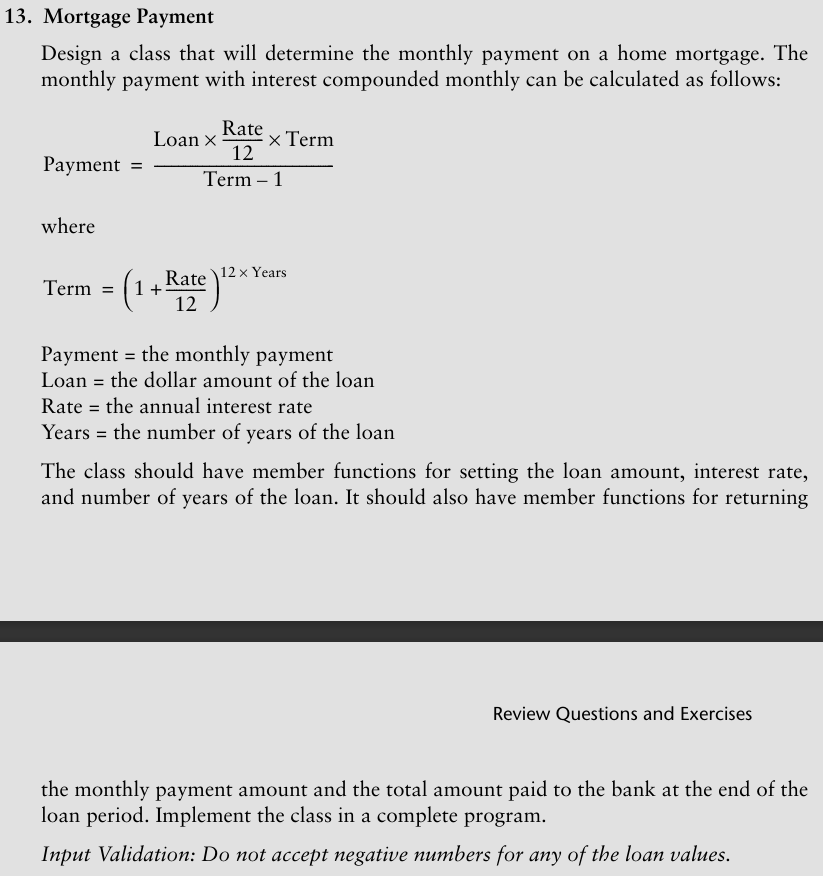
\includegraphics[width=0.8\textwidth]{./Assets/Task requirements/Assignment10/13.13.png}
    \caption{13.13 Task Requirement}
\end{figure}

\subsubsection*{13.13. C++}
\begin{lstlisting}[language=C++, caption=Mortage.cpp]
#include <iostream>
#include <cmath>
#include "Mortgage.h"

using namespace std;

Mortgage::Mortgage(double loan, double rate, int years) {
    this->loan = loan;
    this->rate = rate;
    this->years = years;
}

void Mortgage::setLoan(double loan) {
    this->loan = loan;
}

void Mortgage::setRate(double rate) {
    this->rate = rate;
}

void Mortgage::setYears(int years) {
    this->years = years;
}

double Mortgage::calculateMonthlyPayment() {
    double monthlyRate = rate / 100 / 12;
    int totalMonths = years * 12;
    double term = pow(1 + monthlyRate, totalMonths);

    double payment = (loan * monthlyRate * term) / (term - 1);
    return payment;
}

double Mortgage::calculateTotalAmountPaid() {
    double monthlyPayment = calculateMonthlyPayment();
    int totalMonths = years * 12;
    return monthlyPayment * totalMonths;
}

void Mortgage::displayLoanDetails() {
    double monthlyPayment = calculateMonthlyPayment();
    double totalPaid = calculateTotalAmountPaid();

    cout << "Loan Amount: $" << loan << endl;
    cout << "Annual Interest Rate: " << rate << "%" << endl;
    cout << "Loan Term: " << years << " years" << endl;
    cout << "Monthly Payment: $" << monthlyPayment << endl;
    cout << "Total Amount Paid: $" << totalPaid << endl;
}
\end{lstlisting}

\begin{lstlisting}[language=C++, caption=Mortage.h]
#ifndef MORTGAGE_H
#define MORTGAGE_H

class Mortgage {
private:
    double loan;
    double rate;
    int years;

public:
    Mortgage(double loan, double rate, int years);

    void setLoan(double loan);
    void setRate(double rate);
    void setYears(int years);

    double calculateMonthlyPayment();
    double calculateTotalAmountPaid();
    void displayLoanDetails();
};

#endif
\end{lstlisting}

\begin{lstlisting}[language=C++, caption=main.cpp]
#include <iostream>
#include "Mortgage.h"
using namespace std;

int main() {
    double loan;
    double rate;
    int years;

    do {
        cout << "Enter the loan amount (positive number): ";
        cin >> loan;
        if (loan <= 0) {
            cout << "Invalid input! Loan amount must be positive." << endl;
        }
    } while (loan <= 0);

    do {
        cout << "Enter the annual interest rate (positive number): ";
        cin >> rate;
        if (rate <= 0) {
            cout << "Invalid input! Interest rate must be positive." << endl;
        }
    } while (rate <= 0);

    do {
        cout << "Enter the number of years of the loan (positive number): ";
        cin >> years;
        if (years <= 0) {
            cout << "Invalid input! Number of years must be positive." << endl;
        }
    } while (years <= 0);

    Mortgage mortgage(loan, rate, years);
    mortgage.displayLoanDetails();

    return 0;
}
\end{lstlisting}

\subsubsection*{13.13. Java}
\begin{lstlisting}[language=Java, caption=Mortage.java]
// Mortgage.java
public class Mortgage {
    private double loan;
    private double rate;
    private int years;

    // Constructor
    public Mortgage(double loan, double rate, int years) {
        this.loan = loan;
        this.rate = rate;
        this.years = years;
    }

    // Setters
    public void setLoan(double loan) {
        this.loan = loan;
    }

    public void setRate(double rate) {
        this.rate = rate;
    }

    public void setYears(int years) {
        this.years = years;
    }

    // Calculate Monthly Payment
    public double calculateMonthlyPayment() {
        double monthlyRate = rate / 100 / 12;
        int totalMonths = years * 12;
        double term = Math.pow(1 + monthlyRate, totalMonths);

        double payment = (loan * monthlyRate * term) / (term - 1);
        return payment;
    }

    // Calculate Total Amount Paid
    public double calculateTotalAmountPaid() {
        double monthlyPayment = calculateMonthlyPayment();
        int totalMonths = years * 12;
        return monthlyPayment * totalMonths;
    }

    // Display Loan Details
    public void displayLoanDetails() {
        double monthlyPayment = calculateMonthlyPayment();
        double totalPaid = calculateTotalAmountPaid();

        System.out.printf("Loan Amount: $%.2f\n", loan);
        System.out.printf("Annual Interest Rate: %.2f%%\n", rate);
        System.out.printf("Loan Term: %d years\n", years);
        System.out.printf("Monthly Payment: $%.2f\n", monthlyPayment);
        System.out.printf("Total Amount Paid: $%.2f\n", totalPaid);
    }
}
\end{lstlisting}

\begin{lstlisting}[language=Java, caption=MortageTest.java]
// MortgageTest.java
import java.util.Scanner;

public class MortgageTest {
    public static void main(String[] args) {
        Scanner scanner = new Scanner(System.in);

        // Input loan amount
        double loan = -1;
        while (loan <= 0) {
            System.out.print("Enter the loan amount (positive number): ");
            loan = scanner.nextDouble();
            if (loan <= 0) {
                System.out.println("Invalid input! Loan amount must be positive.");
            }
        }

        // Input interest rate
        double rate = -1;
        while (rate <= 0) {
            System.out.print("Enter the annual interest rate (positive number): ");
            rate = scanner.nextDouble();
            if (rate <= 0) {
                System.out.println("Invalid input! Interest rate must be positive.");
            }
        }

        // Input number of years
        int years = -1;
        while (years <= 0) {
            System.out.print("Enter the number of years of the loan (positive number): ");
            years = scanner.nextInt();
            if (years <= 0) {
                System.out.println("Invalid input! Number of years must be positive.");
            }
        }

        // Create mortgage object and display details
        Mortgage mortgage = new Mortgage(loan, rate, years);
        mortgage.displayLoanDetails();

        scanner.close();
    }
}
\end{lstlisting}

\section*{Assignment 11}

\textbf{Contributor}: Nguyen Duy Duc - 1624838

\subsection*{Java}

\subsubsection*{8.1}

\begin{figure}[H]
    \centering
    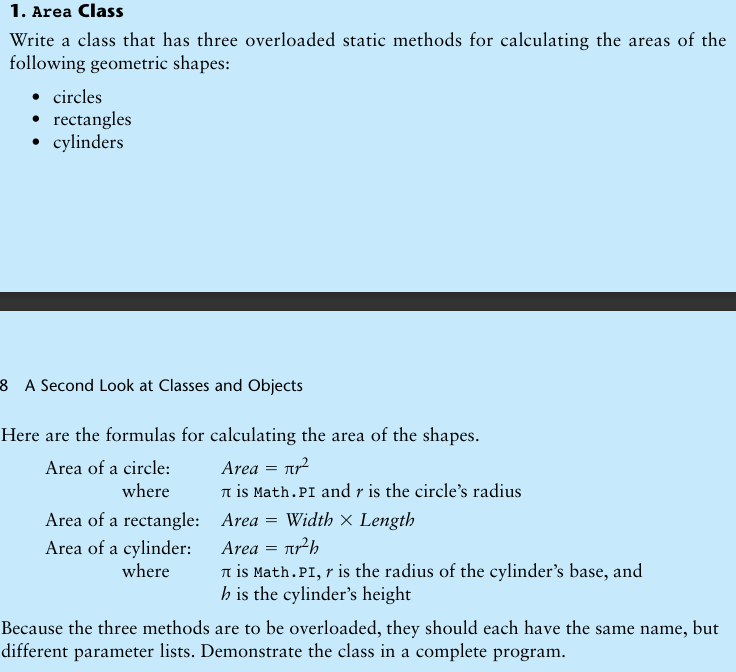
\includegraphics[width=0.8\textwidth]{./Assets/Task requirements/Assignment11/8.1.png}
    \caption{8.1 Task Requirement}
\end{figure}

\begin{lstlisting}[caption=Area.java]
public class Area {

    // Area of a circle
    public static double calculateArea(double radius) {
        return Math.PI * radius * radius;
    }

    // Area of a rectangle
    public static double calculateArea(double width, double length) {
        return width * length;
    }

    // Area of a cylinder
    public static double calculateArea(double radius, double height, boolean isCylinder) {
        return Math.PI * radius * radius * height;
    }
}
\end{lstlisting}

\begin{lstlisting}[caption=AreaDemo.java]
import java.util.Scanner;

public class AreaDemo {
    public static void main(String[] args) {
        Scanner scanner = new Scanner(System.in);

        System.out.println("Select a shape to calculate the area:");
        System.out.println("1. Circle");
        System.out.println("2. Rectangle");
        System.out.println("3. Cylinder");

        int choice = scanner.nextInt();

        switch (choice) {
            case 1:
                // Circle
                System.out.print("Enter the radius of the circle: ");
                double radiusCircle = scanner.nextDouble();
                double circleArea = Area.calculateArea(radiusCircle);
                System.out.printf("The area of the circle is: %.2f\n", circleArea);
                break;

            case 2:
                // Rectangle
                System.out.print("Enter the width of the rectangle: ");
                double width = scanner.nextDouble();
                System.out.print("Enter the length of the rectangle: ");
                double length = scanner.nextDouble();
                double rectangleArea = Area.calculateArea(width, length);
                System.out.printf("The area of the rectangle is: %.2f\n", rectangleArea);
                break;

            case 3:
                // Cylinder
                System.out.print("Enter the radius of the cylinder: ");
                double radiusCylinder = scanner.nextDouble();
                System.out.print("Enter the height of the cylinder: ");
                double height = scanner.nextDouble();
                double cylinderArea = Area.calculateArea(radiusCylinder, height, true);
                System.out.printf("The area of the cylinder is: %.2f\n", cylinderArea);
                break;

            default:
                System.out.println("Invalid choice! Please select 1, 2, or 3.");
        }

        scanner.close();
    }
}
\end{lstlisting}

\subsubsection*{8.2}

\begin{figure}[H]
    \centering
    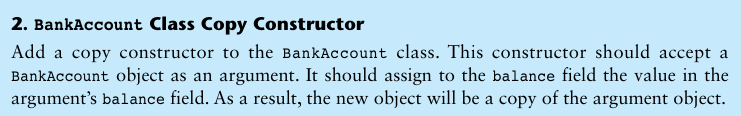
\includegraphics[width=0.8\textwidth]{./Assets/Task requirements/Assignment11/8.2.png}
    \caption{8.2 Task Requirement}
\end{figure}

\begin{lstlisting}[caption=BankAccount.java]
public class BankAccount {
    private double balance;

    // Constructor
    public BankAccount(double initialBalance) {
        balance = initialBalance;
    }

    // Copy constructor
    public BankAccount(BankAccount account) {
        this.balance = account.balance;
    }

    public double getBalance() {
        return balance;
    }

    public void deposit(double amount) {
        balance += amount;
    }

    public void withdraw(double amount) {
        if (amount <= balance) {
            balance -= amount;
        } else {
            System.out.println("Insufficient funds.");
        }
    }

    public static void main(String[] args) {
        // Create a BankAccount object
        BankAccount account1 = new BankAccount(1000.0);

        // Create a copy of account1
        BankAccount account2 = new BankAccount(account1);

        // Display the balances
        System.out.println("Balance of account1: " + account1.getBalance());
        System.out.println("Balance of account2: " + account2.getBalance());
    }
}
\end{lstlisting}

\subsubsection*{8.3}

\begin{figure}[H]
    \centering
    \includegraphics[width=0.8\textwidth]{./Assets/Task requirements/Assignment11/8.3.png}
    \caption{8.3 Task Requirement}
\end{figure}

\begin{lstlisting}[caption=CarpetCalculator.java]
import java.util.Scanner;

public class CarpetCalculator {
    public static void main(String[] args) {
        Scanner scanner = new Scanner(System.in);

        // Get the dimensions
        System.out.print("Enter the length of the room in feet: ");
        double length = scanner.nextDouble();

        System.out.print("Enter the width of the room in feet: ");
        double width = scanner.nextDouble();

        // Create a RoomDimension object
        RoomDimension roomDimension = new RoomDimension(length, width);

        // Get the cost per square foot of the carpet
        System.out.print("Enter the cost per square foot of the carpet: ");
        double costPerSquareFoot = scanner.nextDouble();

        // Create a RoomCarpet object
        RoomCarpet roomCarpet = new RoomCarpet(roomDimension, costPerSquareFoot);

        // Display the total cost
        System.out.println("The total cost of the carpet: $" + roomCarpet.getTotalCost());
    }
}
\end{lstlisting}

\begin{lstlisting}[caption=RoomCarpet.java]
class RoomCarpet {
    private RoomDimension dimension;
    private double costPerSquareFoot;

    // Constructor
    public RoomCarpet(RoomDimension dimension, double costPerSquareFoot) {
        this.dimension = dimension;
        this.costPerSquareFoot = costPerSquareFoot;
    }

    public double getTotalCost() {
        return dimension.getArea() * costPerSquareFoot;
    }
}
\end{lstlisting}

\begin{lstlisting}[caption=RoomDimension.java]
class RoomDimension {
    private double length;
    private double width;

    // Constructor
    public RoomDimension(double length, double width) {
        this.length = length;
        this.width = width;
    }

    public double getArea() {
        return length * width;
    }
}
\end{lstlisting}

\subsection*{C++}

\subsubsection*{14.1}

\begin{figure}[H]
    \centering
    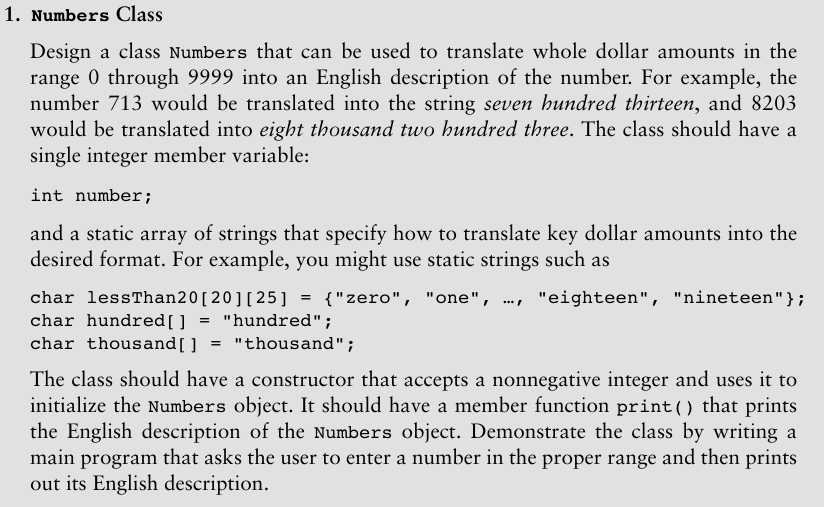
\includegraphics[width=0.8\textwidth]{./Assets/Task requirements/Assignment11/14.1.png}
    \caption{14.1 Task Requirement}
\end{figure}

\begin{lstlisting}[caption=Numbers.cpp]
#include <iostream>
#include <string>

using namespace std;

class Numbers {
private:
    int number;
    static string lessThan20[20];
    static string tens[10];
    static string hundred;
    static string thousand;

public:
    // Constructor
    Numbers(int num) : number(num) {}

    // Function to print the English description of the number
    void print() const {
        if (number == 0) {
            cout << lessThan20[0] << endl;
            return;
        }

        string result;
        int tempNumber = number;

        if (tempNumber >= 1000) {
            result += lessThan20[tempNumber / 1000] + " " + thousand + " ";
            tempNumber %= 1000;
        }
        if (tempNumber >= 100) {
            result += lessThan20[tempNumber / 100] + " " + hundred + " ";
            tempNumber %= 100;
        }
        if (tempNumber >= 20) {
            result += tens[tempNumber / 10] + " ";
            tempNumber %= 10;
        }
        if (tempNumber > 0) {
            result += lessThan20[tempNumber] + " ";
        }

        cout << result << endl;
    }
};

// Static member initialization
string Numbers::lessThan20[20] = {"zero", "one", "two", "three", "four", "five", "six", "seven", "eight", "nine", "ten", "eleven", "twelve", "thirteen", "fourteen", "fifteen", "sixteen", "seventeen", "eighteen", "nineteen"};
string Numbers::tens[10] = {"", "", "twenty", "thirty", "forty", "fifty", "sixty", "seventy", "eighty", "ninety"};
string Numbers::hundred = "hundred";
string Numbers::thousand = "thousand";

int main() {
    int num;

    // Loop until a valid number is entered
    do {
        cout << "Enter a number between 0 and 9999: ";
        cin >> num;

        if (num < 0 || num > 9999) {
            cout << "Number out of range! Please try again." << endl;
        }
    } while (num < 0 || num > 9999);

    Numbers number(num);
    number.print();

    return 0;
}
\end{lstlisting}

\subsubsection*{14.2}

\begin{figure}[H]
    \centering
    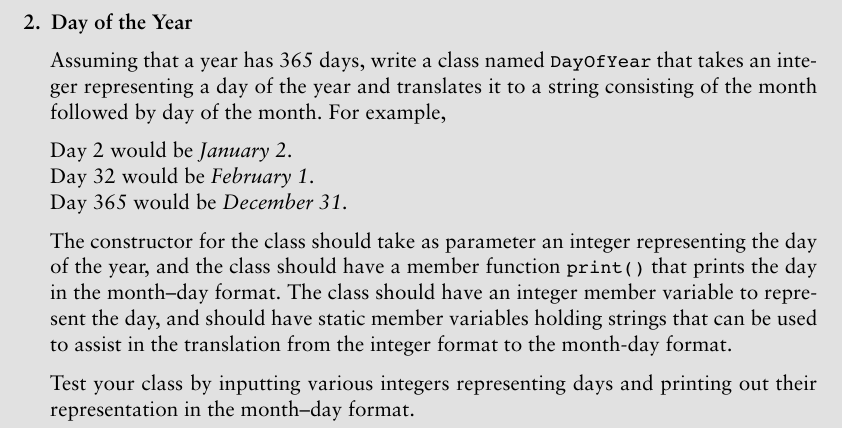
\includegraphics[width=0.8\textwidth]{./Assets/Task requirements/Assignment11/14.2.png}
    \caption{14.2 Task Requirement}
\end{figure}

\begin{lstlisting}[caption=DayOfYear.cpp]
#include <iostream>
#include <string>

using namespace std;

class DayOfYear {
private:
    int day;
    static string months[12];
    static int daysInMonth[12];

public:
    // Constructor
    DayOfYear(int dayOfYear) : day(dayOfYear) {}

    // Function to print the day in month-day format
    void print() const {
        int month = 0;
        int dayOfMonth = day;

        while (dayOfMonth > daysInMonth[month]) {
            dayOfMonth -= daysInMonth[month];
            month++;
        }

        cout << months[month] << " " << dayOfMonth << endl;
    }
};

// Static member initialization
string DayOfYear::months[12] = {"January", "February", "March", "April", "May", "June", "July", "August", "September", "October", "November", "December"};
int DayOfYear::daysInMonth[12] = {31, 28, 31, 30, 31, 30, 31, 31, 30, 31, 30, 31};

int main() {
    int dayOfYear;

    // Loop until a valid day is entered
    do {
        cout << "Enter a day of the year (1-365): ";
        cin >> dayOfYear;

        if (dayOfYear < 1 || dayOfYear > 365) {
            cout << "Day out of range! Please try again." << endl;
        }
    } while (dayOfYear < 1 || dayOfYear > 365);

    DayOfYear day(dayOfYear);
    day.print();

    return 0;
}
\end{lstlisting}

\section*{Assignment 12}

\textbf{Contributor}: Ngo Thanh Trung - 1677469

\subsection*{Java}

\subsubsection*{8.3}

\begin{figure}[H]
    \centering
    \includegraphics[width=0.8\textwidth]{./Assets/Task requirements/Assignment12/8.3.png}
    \caption{8.3 Task Requirement}
\end{figure}

\begin{lstlisting}[caption=CarpetCalculator.java]
package carpetCalculator.Code;
import java.util.Scanner;

public class CarpetCalculator {
    public static void main(String[] args) {
    Scanner sc = new Scanner(System.in);

    System.out.print("Enter the length of the room (m): ");
    double length = sc.nextDouble();
    System.out.print("Enter the width of the room (m): ");
    double width = sc.nextDouble();

    RoomDimension myRoom = new RoomDimension(length, width);
    System.out.println("Room entered area (m^2): " + myRoom.getRoomArea());

    System.out.print("Enter the price per square (₫): ");
    double pricePerSquare = sc.nextDouble();

    RoomCarpet myCarpet = new RoomCarpet(myRoom, pricePerSquare);
    System.out.println("Price for " + myRoom.getRoomArea() + " room area: " + myCarpet.getTotalCost() + "₫");
    }
}
\end{lstlisting}

\begin{lstlisting}[caption=RoomCarpet.java]
package carpetCalculator.Code;

public class RoomCarpet {
    private RoomDimension roomDimension;
    private double costPerSqF = 0;

    public RoomCarpet(RoomDimension roomDimension, double costPerSqF) {
        this.roomDimension = roomDimension;
        if (costPerSqF > 0) {
            this.costPerSqF = costPerSqF;
        }
    }

    public double getTotalCost() {
        return costPerSqF * roomDimension.getRoomArea();
    }
}
\end{lstlisting}

\begin{lstlisting}[caption=RoomDimension.java]
package carpetCalculator.Code;

public class RoomDimension {
    private double roomLength = 0;
    private double roomWidth = 0;

    RoomDimension(double roomLength, double roomWidth) {
        if (roomLength > 0) {
            this.roomLength = roomLength;
        }
        if (roomWidth > 0) {
            this.roomWidth = roomWidth;
        }
    }

    public double getRoomArea() {
        return roomLength * roomWidth;
    }
}
\end{lstlisting}

\begin{figure}[H]
    \centering
    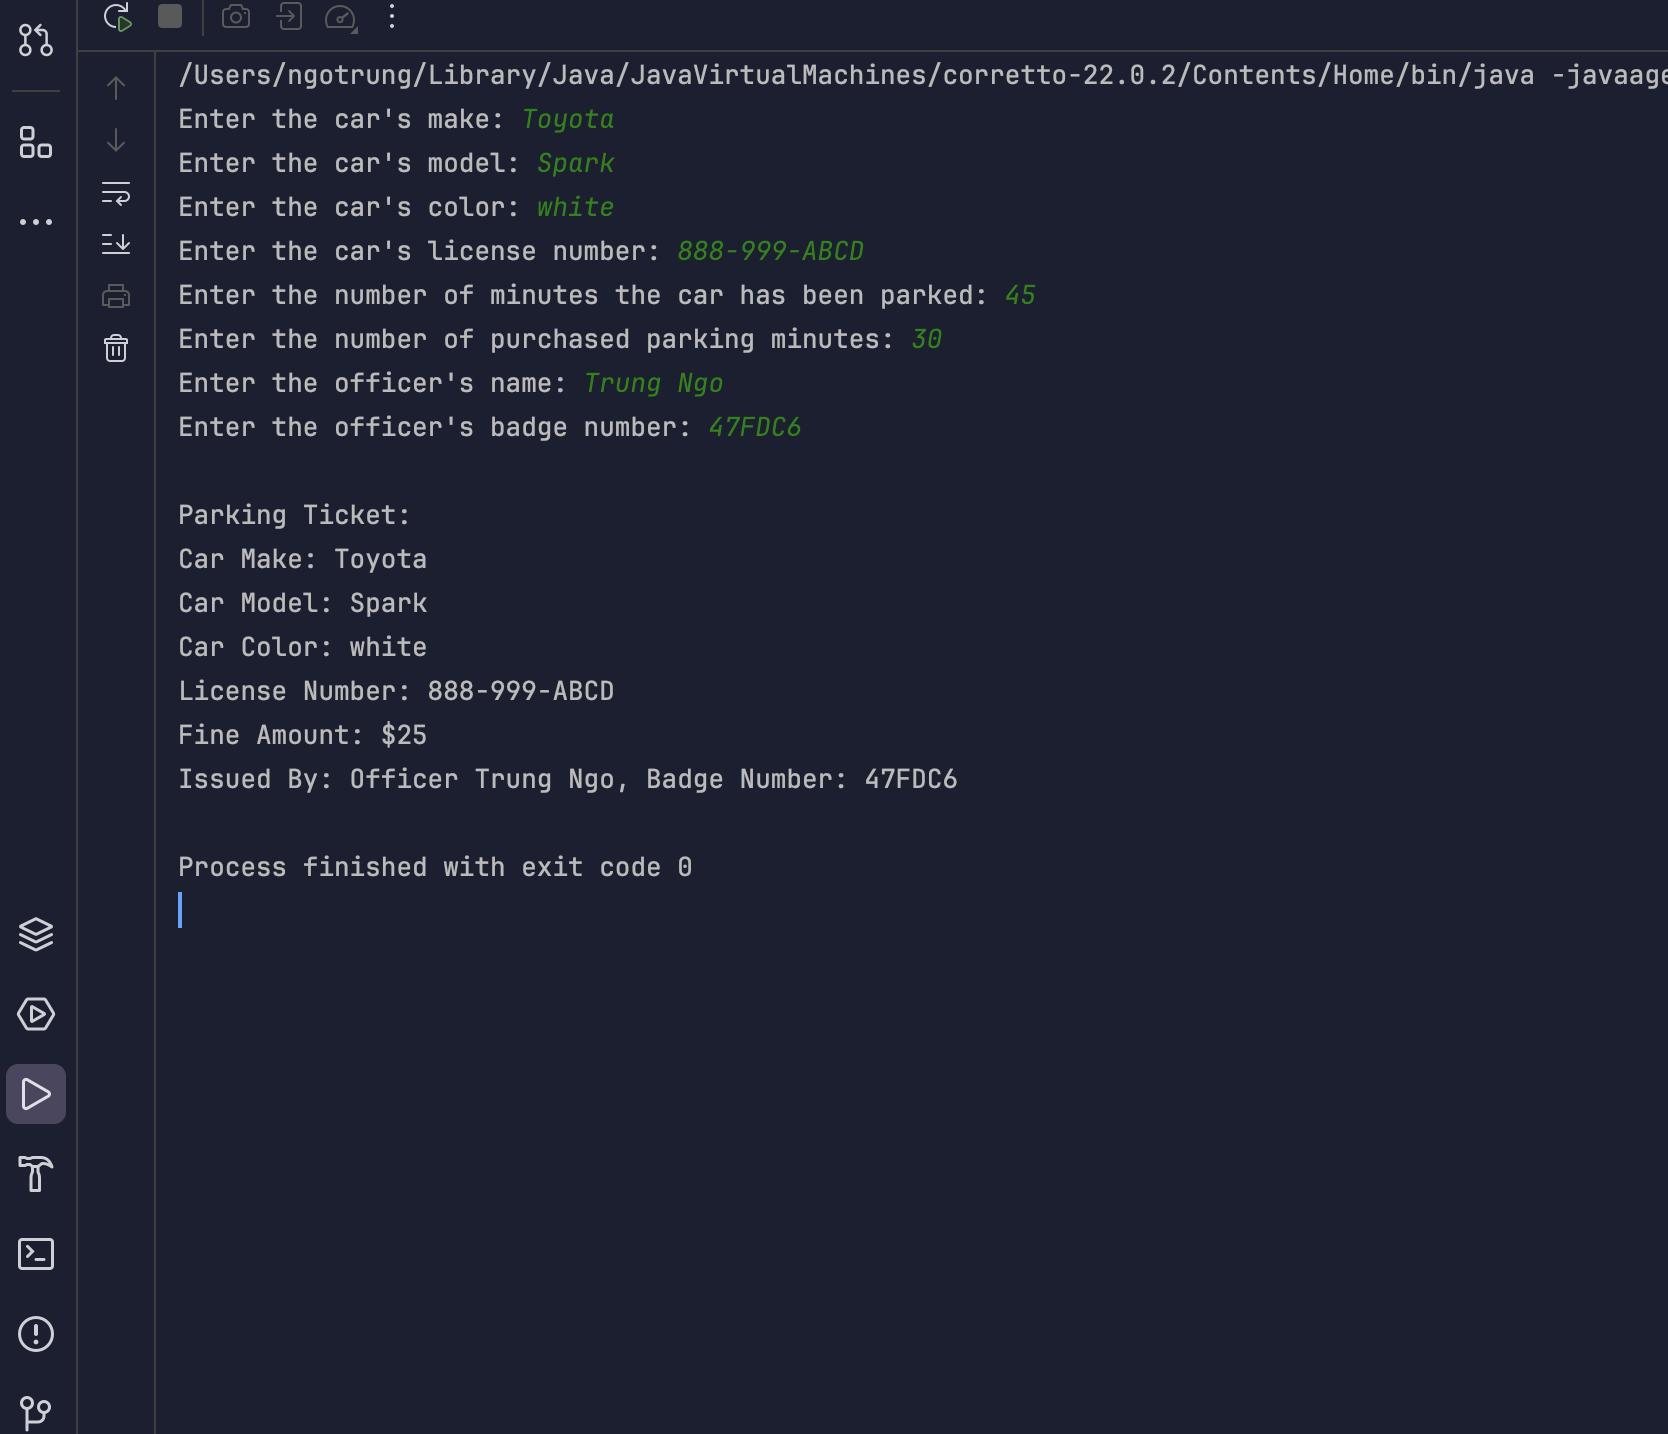
\includegraphics[width=0.8\textwidth]{./Assets/Results/Assignment12/1.png}
    \caption{8.3 Result}
\end{figure}

\subsubsection*{8.8}

\begin{figure}[H]
    \centering
    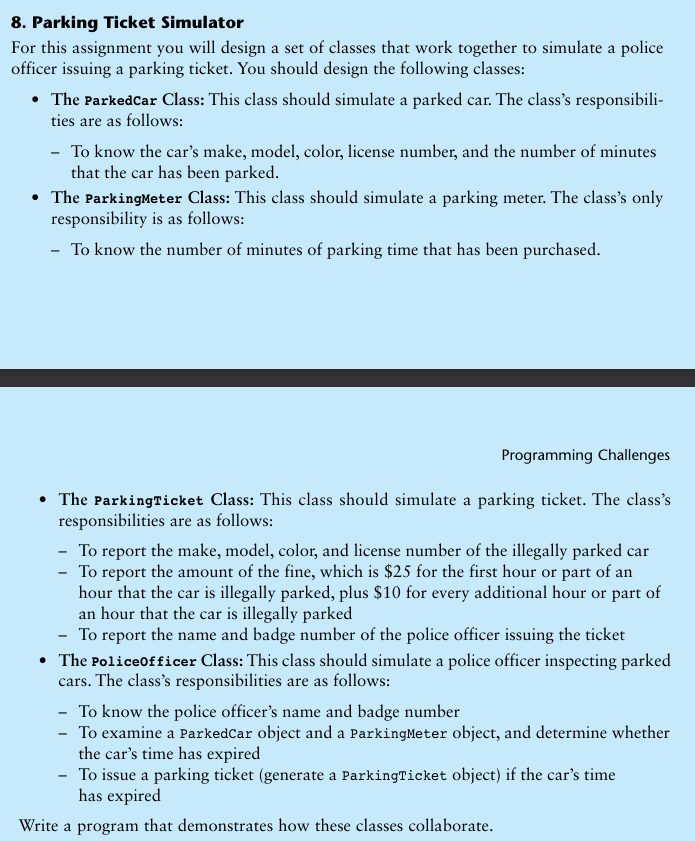
\includegraphics[width=0.8\textwidth]{./Assets/Task requirements/Assignment12/8.8.png}
    \caption{8.8 Task Requirement}
\end{figure}

\begin{lstlisting}[caption=ParkedCar.java]
package Code;

public class ParkedCar {
    private String make;
    private String model;
    private String color;
    private String licenseNumber;
    private int parkedMinutes;

    public ParkedCar(String make, String model, String color, String licenseNumber, int parkedMinutes) {
        this.make = make;
        this.model = model;
        this.color = color;
        this.licenseNumber = licenseNumber;
        if (parkedMinutes >= 0) {
            this.parkedMinutes = parkedMinutes;
        } else {
            this.parkedMinutes = 0;
        }
    }

    public String getMake() {
        return make;
    }

    public String getModel() {
        return model;
    }

    public String getColor() {
        return color;
    }

    public String getLicenseNumber() {
        return licenseNumber;
    }

    public int getParkedMinutes() {
        return parkedMinutes;
    }
}
\end{lstlisting}

\begin{lstlisting}[caption=ParkingMeter.java]
package Code;

public class ParkingMeter {
    private int purchasedMinutes;

    public ParkingMeter(int purchasedMinutes) {
        if (purchasedMinutes >= 0) {
            this.purchasedMinutes = purchasedMinutes;
        } else {
            this.purchasedMinutes = 0;
        }
    }

    public int getPurchasedMinutes() {
        return purchasedMinutes;
    }
}
\end{lstlisting}

\begin{lstlisting}[caption=ParkingTicket.java]
package Code;

public class ParkingTicket {
    private String carMake;
    private String carModel;
    private String carColor;
    private String licenseNumber;
    private String officerName;
    private String officerBadgeNumber;
    private int fine;

    public ParkingTicket(ParkedCar car, String officerName, String officerBadgeNumber, int overParkedMinutes) {
        this.carMake = car.getMake();
        this.carModel = car.getModel();
        this.carColor = car.getColor();
        this.licenseNumber = car.getLicenseNumber();
        this.officerName = officerName;
        this.officerBadgeNumber = officerBadgeNumber;

        calculateFine(overParkedMinutes);
    }

    private void calculateFine(int overParkedMinutes) {
        int hours = (int) Math.ceil(overParkedMinutes / 60.0);
        fine = 25 + (hours - 1) * 10;
    }

    public String getTicketDetails() {
        return  "\n" +
                "Parking Ticket:\n" +
                "Car Make: " + carMake + "\n" +
                "Car Model: " + carModel + "\n" +
                "Car Color: " + carColor + "\n" +
                "License Number: " + licenseNumber + "\n" +
                "Fine Amount: $" + fine + "\n" +
                "Issued By: Officer " + officerName + ", Badge Number: " + officerBadgeNumber;
    }
}
\end{lstlisting}

\begin{lstlisting}[caption=ParkingTicketSimulator.java]
package Code;

import java.util.Scanner;

public class ParkingTicketSimulator {
    public static void main(String[] args) {
        Scanner sc = new Scanner(System.in);

        System.out.print("Enter the car's make: ");
        String make = sc.nextLine();
        System.out.print("Enter the car's model: ");
        String model = sc.nextLine();
        System.out.print("Enter the car's color: ");
        String color = sc.nextLine();
        System.out.print("Enter the car's license number: ");
        String licenseNumber = sc.nextLine();
        System.out.print("Enter the number of minutes the car has been parked: ");
        int parkedMinutes = sc.nextInt();

        ParkedCar car = new ParkedCar(make, model, color, licenseNumber, parkedMinutes);

        System.out.print("Enter the number of purchased parking minutes: ");
        int purchasedMinutes = sc.nextInt();
        ParkingMeter meter = new ParkingMeter(purchasedMinutes);

        System.out.print("Enter the officer's name: ");
        sc.nextLine();
        String officerName = sc.nextLine();
        System.out.print("Enter the officer's badge number: ");
        String badgeNumber = sc.nextLine();
        PoliceOfficer officer = new PoliceOfficer(officerName, badgeNumber);

        ParkingTicket ticket = officer.inspectCar(car, meter);
        if (ticket != null) {
            System.out.println(ticket.getTicketDetails());
        } else {
            System.out.println("No ticket issued. The car is legally parked.");
        }

        sc.close();
    }
}
\end{lstlisting}

\begin{lstlisting}[caption=PoliceOfficer.java]
package Code;

public class PoliceOfficer {
    private String name;
    private String badgeNumber;

    public PoliceOfficer(String name, String badgeNumber) {
        this.name = name;
        this.badgeNumber = badgeNumber;
    }

    public ParkingTicket inspectCar(ParkedCar car, ParkingMeter meter) {
        int overParkedMinutes = car.getParkedMinutes() - meter.getPurchasedMinutes();
        if (overParkedMinutes > 0) {
            return new ParkingTicket(car, name, badgeNumber, overParkedMinutes);
        }
        return null;
    }
}
\end{lstlisting}

\begin{figure}[H]
    \centering
    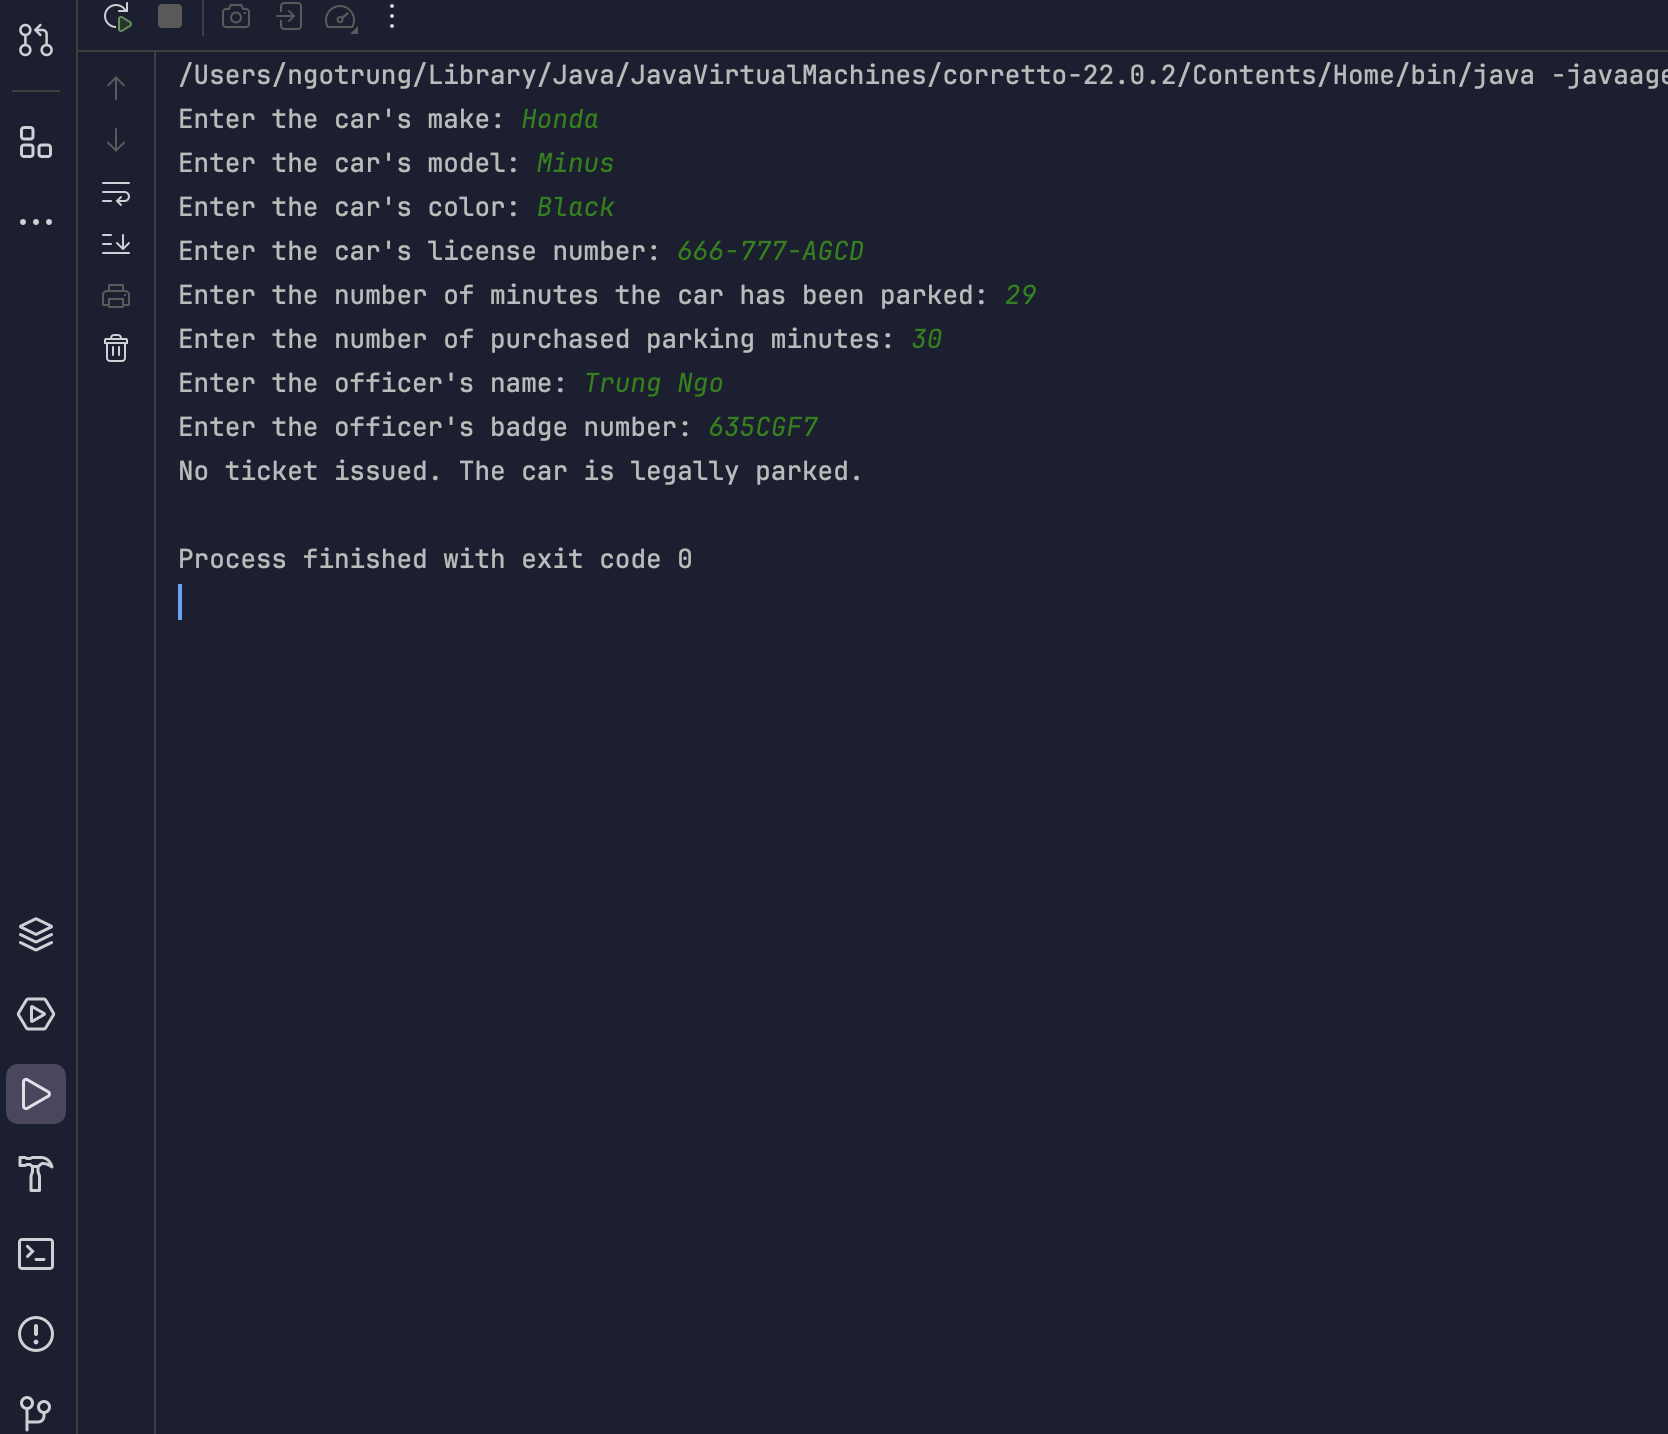
\includegraphics[width=0.8\textwidth]{./Assets/Results/Assignment12/2.png}
    \caption{8.8 Result}
\end{figure}

\subsection*{C++}

\subsubsection*{14.13}

\begin{figure}[H]
    \centering
    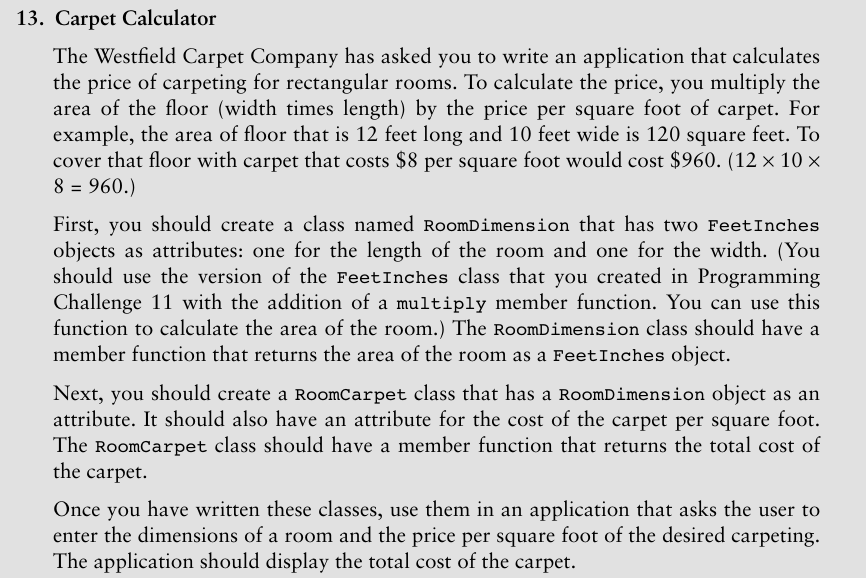
\includegraphics[width=0.8\textwidth]{./Assets/Task requirements/Assignment12/14.13.png}
    \caption{14.13 Task Requirement}
\end{figure}

\begin{lstlisting}[language=C++, caption={FeetInches.h}]
#ifndef FEETINCHES_H
#define FEETINCHES_H

class FeetInches {
private:
    int feet;
    int inches;
    void normalize();
public:
    FeetInches(int ft = 0, int in = 0);
    int getFeet() const;
    int getInches() const;
    double multiply(const FeetInches& other) const;
    void display() const;
};

#endif
\end{lstlisting}

\begin{lstlisting}[language=C++, caption={FeetInches.cpp}]
#include "FeetInches.h"
#include <cmath>
#include <iostream>

FeetInches::FeetInches(int ft, int in) : feet(ft), inches(in) {
    normalize();
}

void FeetInches::normalize() {
    if (inches >= 12) {
        feet += inches / 12;
        inches %= 12;
    } else if (inches < 0) {
        feet -= (std::abs(inches) / 12) + 1;
        inches = 12 - (std::abs(inches) % 12);
    }
}

int FeetInches::getFeet() const {
    return feet;
}

int FeetInches::getInches() const {
    return inches;
}

double FeetInches::multiply(const FeetInches& other) const {
    double thisFeet = feet + inches / 12.0;
    double otherFeet = other.feet + other.inches / 12.0;
    return thisFeet * otherFeet;
}

void FeetInches::display() const {
    std::cout << feet << " feet " << inches << " inches";
}
\end{lstlisting}

\begin{lstlisting}[language=C++, caption={RoomDimension.h}]
#ifndef ROOMDIMENSION_H
#define ROOMDIMENSION_H

#include "FeetInches.h"

class RoomDimension {
private:
    FeetInches length;
    FeetInches width;
public:
    RoomDimension(const FeetInches& len, const FeetInches& wid);
    FeetInches getLength() const;
    FeetInches getWidth() const;
    double getArea() const;
    void display() const;
};

#endif
\end{lstlisting}

\begin{lstlisting}[language=C++, caption={RoomDimension.cpp}]
#include "RoomDimension.h"
#include <iostream>

RoomDimension::RoomDimension(const FeetInches& len, const FeetInches& wid)
    : length(len), width(wid) {}

FeetInches RoomDimension::getLength() const {
    return length;
}

FeetInches RoomDimension::getWidth() const {
    return width;
}

double RoomDimension::getArea() const {
    return length.multiply(width);
}

void RoomDimension::display() const {
    std::cout << "Length: ";
    length.display();
    std::cout << ", Width: ";
    width.display();
}
\end{lstlisting}

\begin{lstlisting}[language=C++, caption={RoomCarpet.h}]
#ifndef ROOMCARPET_H
#define ROOMCARPET_H

#include "RoomDimension.h"

class RoomCarpet {
private:
    RoomDimension room;
    double costPerSquareFoot;
public:
    RoomCarpet(const RoomDimension& rd, double cost);
    double getTotalCost() const;
};

#endif
\end{lstlisting}

\begin{lstlisting}[language=C++, caption={RoomCarpet.cpp}]
#include "RoomCarpet.h"
#include <iostream>
#include <iomanip>

RoomCarpet::RoomCarpet(const RoomDimension& rd, double cost)
    : room(rd), costPerSquareFoot(cost) {}

double RoomCarpet::getTotalCost() const {
    return room.getArea() * costPerSquareFoot;
}
\end{lstlisting}

\begin{lstlisting}[language=C++, caption={main.cpp}]
#include <iostream>
#include <iomanip>
#include "FeetInches.h"
#include "RoomDimension.h"
#include "RoomCarpet.h"

int main() {
    int lengthFeet, lengthInches;
    int widthFeet, widthInches;
    double pricePerSqFt;

    std::cout << "Enter the length of the room.\n";
    std::cout << "Feet: ";
    std::cin >> lengthFeet;
    std::cout << "Inches: ";
    std::cin >> lengthInches;

    std::cout << "\nEnter the width of the room.\n";
    std::cout << "Feet: ";
    std::cin >> widthFeet;
    std::cout << "Inches: ";
    std::cin >> widthInches;

    std::cout << "\nEnter the price of the carpet per square foot: $";
    std::cin >> pricePerSqFt;

    FeetInches length(lengthFeet, lengthInches);
    FeetInches width(widthFeet, widthInches);
    RoomDimension room(length, width);
    RoomCarpet carpet(room, pricePerSqFt);

    double area = room.getArea();
    double totalCost = carpet.getTotalCost();

    std::cout << "\nRoom Dimensions:\n";
    room.display();
    std::cout << "\nArea: " << std::fixed << std::setprecision(2) << area << " square feet";
    std::cout << "\nTotal cost of " << area << " area: $" << totalCost << "\n";

    return 0;
}
}
\end{lstlisting}

\begin{figure}[H]
    \centering
    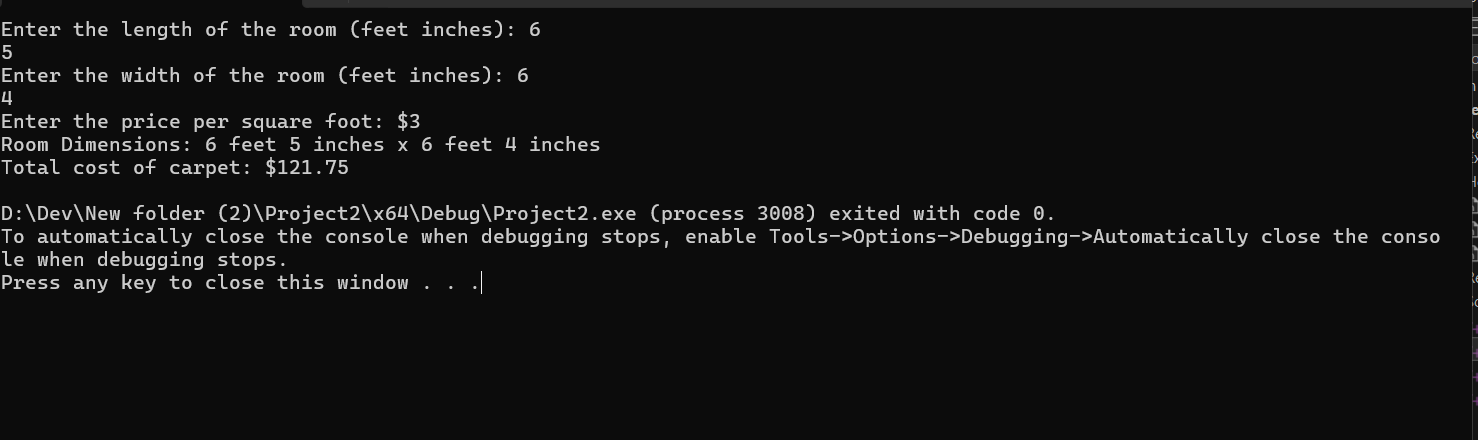
\includegraphics[width=0.8\textwidth]{./Assets/Results/Assignment12/3.png}
    \caption{14.13 Result}
\end{figure}

\subsubsection*{14.14}

\begin{figure}[H]
    \centering
    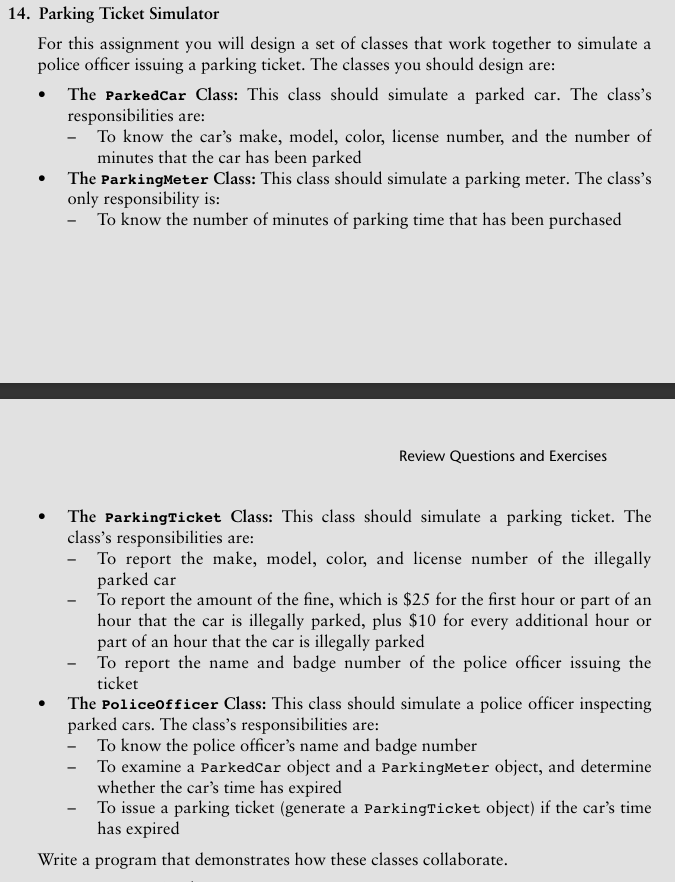
\includegraphics[width=0.8\textwidth]{./Assets/Task requirements/Assignment12/14.14.png}
    \caption{14.14 Task Requirement}
\end{figure}

\begin{lstlisting}[language=C++, caption={ParkedCar.h}]
#ifndef PARKEDCAR_H
#define PARKEDCAR_H

#include <string>
using namespace std;

class ParkedCar {
private:
    string make;
    string model;
    string color;
    string licenseNumber;
    int parkedMinutes;

public:
    ParkedCar(const string& carMake, const string& carModel, const string& carColor, const string& license, int minutesParked);
    string getMake() const;
    string getModel() const;
    string getColor() const;
    string getLicenseNumber() const;
    int getParkedMinutes() const;
};

#endif
\end{lstlisting}

\begin{lstlisting}[language=C++, caption={ParkingMeter.h}]
#ifndef PARKINGMETER_H
#define PARKINGMETER_H

#include <string>
using namespace std;

class ParkingMeter {
private:
    int purchasedMinutes;

public:
    ParkingMeter(int minutesPurchased);
    int getPurchasedMinutes() const;
};

#endif
\end{lstlisting}

\begin{lstlisting}[language=C++, caption={ParkingTicket.h}]
#ifndef PARKINGTICKET_H
#define PARKINGTICKET_H

#include "ParkedCar.h"
#include <string>
using namespace std;

class ParkingTicket {
private:
    string carMake;
    string carModel;
    string carColor;
    string licenseNumber;
    string officerName;
    string officerBadgeNumber;
    int fine;
    void calculateFine(int overParkedMinutes);

public:
    ParkingTicket(const ParkedCar& car, const string& officer, const string& badge, int overParkedMinutes);
    void printTicket() const;
};

#endif
\end{lstlisting}

\begin{lstlisting}[language=C++, caption={PoliceOfficer.h}]
#ifndef POLICEOFFICER_H
#define POLICEOFFICER_H

#include "ParkedCar.h"
#include "ParkingMeter.h"
#include "ParkingTicket.h"
#include <string>
using namespace std;

class PoliceOfficer {
private:
    string name;
    string badgeNumber;

public:
    PoliceOfficer(const string& officerName, const string& badge);
    ParkingTicket* inspectCar(const ParkedCar& car, const ParkingMeter& meter) const;
};

#endif
\end{lstlisting}

\begin{lstlisting}[language=C++, caption={ParkingTicket.cpp}]
#include "ParkingTicket.h"
#include <iostream>
#include <cmath>

ParkingTicket::ParkingTicket(const ParkedCar& car, const string& officer, const string& badge, int overParkedMinutes)
    : carMake(car.getMake()), carModel(car.getModel()), carColor(car.getColor()),
      licenseNumber(car.getLicenseNumber()), officerName(officer), officerBadgeNumber(badge) {
    calculateFine(overParkedMinutes);
}

void ParkingTicket::calculateFine(int overParkedMinutes) {
    int hours = static_cast<int>(ceil(overParkedMinutes / 60.0)); // rounding up
    fine = 25 + (hours - 1) * 10;
}

void ParkingTicket::printTicket() const {
    std::cout << "Parking Ticket:\n"
              << "Car Make: " << carMake << "\n"
              << "Car Model: " << carModel << "\n"
              << "Car Color: " << carColor << "\n"
              << "License Number: " << licenseNumber << "\n"
              << "Fine Amount: $" << fine << "\n"
              << "Issued By: Officer " << officerName << " (Badge " << officerBadgeNumber << ")\n";
}
\end{lstlisting}

\begin{lstlisting}[language=C++, caption={PoliceOfficer.cpp}]
#include "PoliceOfficer.h"

PoliceOfficer::PoliceOfficer(const string& officerName, const string& badge) : name(officerName), badgeNumber(badge) {}

ParkingTicket* PoliceOfficer::inspectCar(const ParkedCar& car, const ParkingMeter& meter) const {
    int overParkedMinutes = car.getParkedMinutes() - meter.getPurchasedMinutes();
    if (overParkedMinutes > 0) {
        return new ParkingTicket(car, name, badgeNumber, overParkedMinutes);
    }
    return nullptr;
}
\end{lstlisting}

\begin{lstlisting}[language=C++, caption={main.cpp}]
#include "ParkedCar.h"
#include "ParkingMeter.h"
#include "ParkingTicket.h"
#include "PoliceOfficer.h"
#include <iostream>
using namespace std;

void checkTicket(const ParkedCar& car, const ParkingMeter& meter, const PoliceOfficer& officer) {
    ParkingTicket* ticket = officer.inspectCar(car, meter);
    if (ticket != nullptr) {
        ticket->printTicket();
        delete ticket;
    } else {
        cout << "No ticket issued. The car is legally parked.\n";
    }
}

int main() {
    ParkedCar carValid("Toyota", "Corona", "White", "ABC123", 59);
    ParkedCar carFined("Toyota", "Corona", "White", "ABC124", 125);
    ParkingMeter meter(60);
    PoliceOfficer officer("Ngo Trung", "342FHCB7");

    checkTicket(carValid, meter, officer);
    cout << "\n";
    checkTicket(carFined, meter, officer);

    return 0;
}
\end{lstlisting}

\begin{figure}[H]
    \centering
    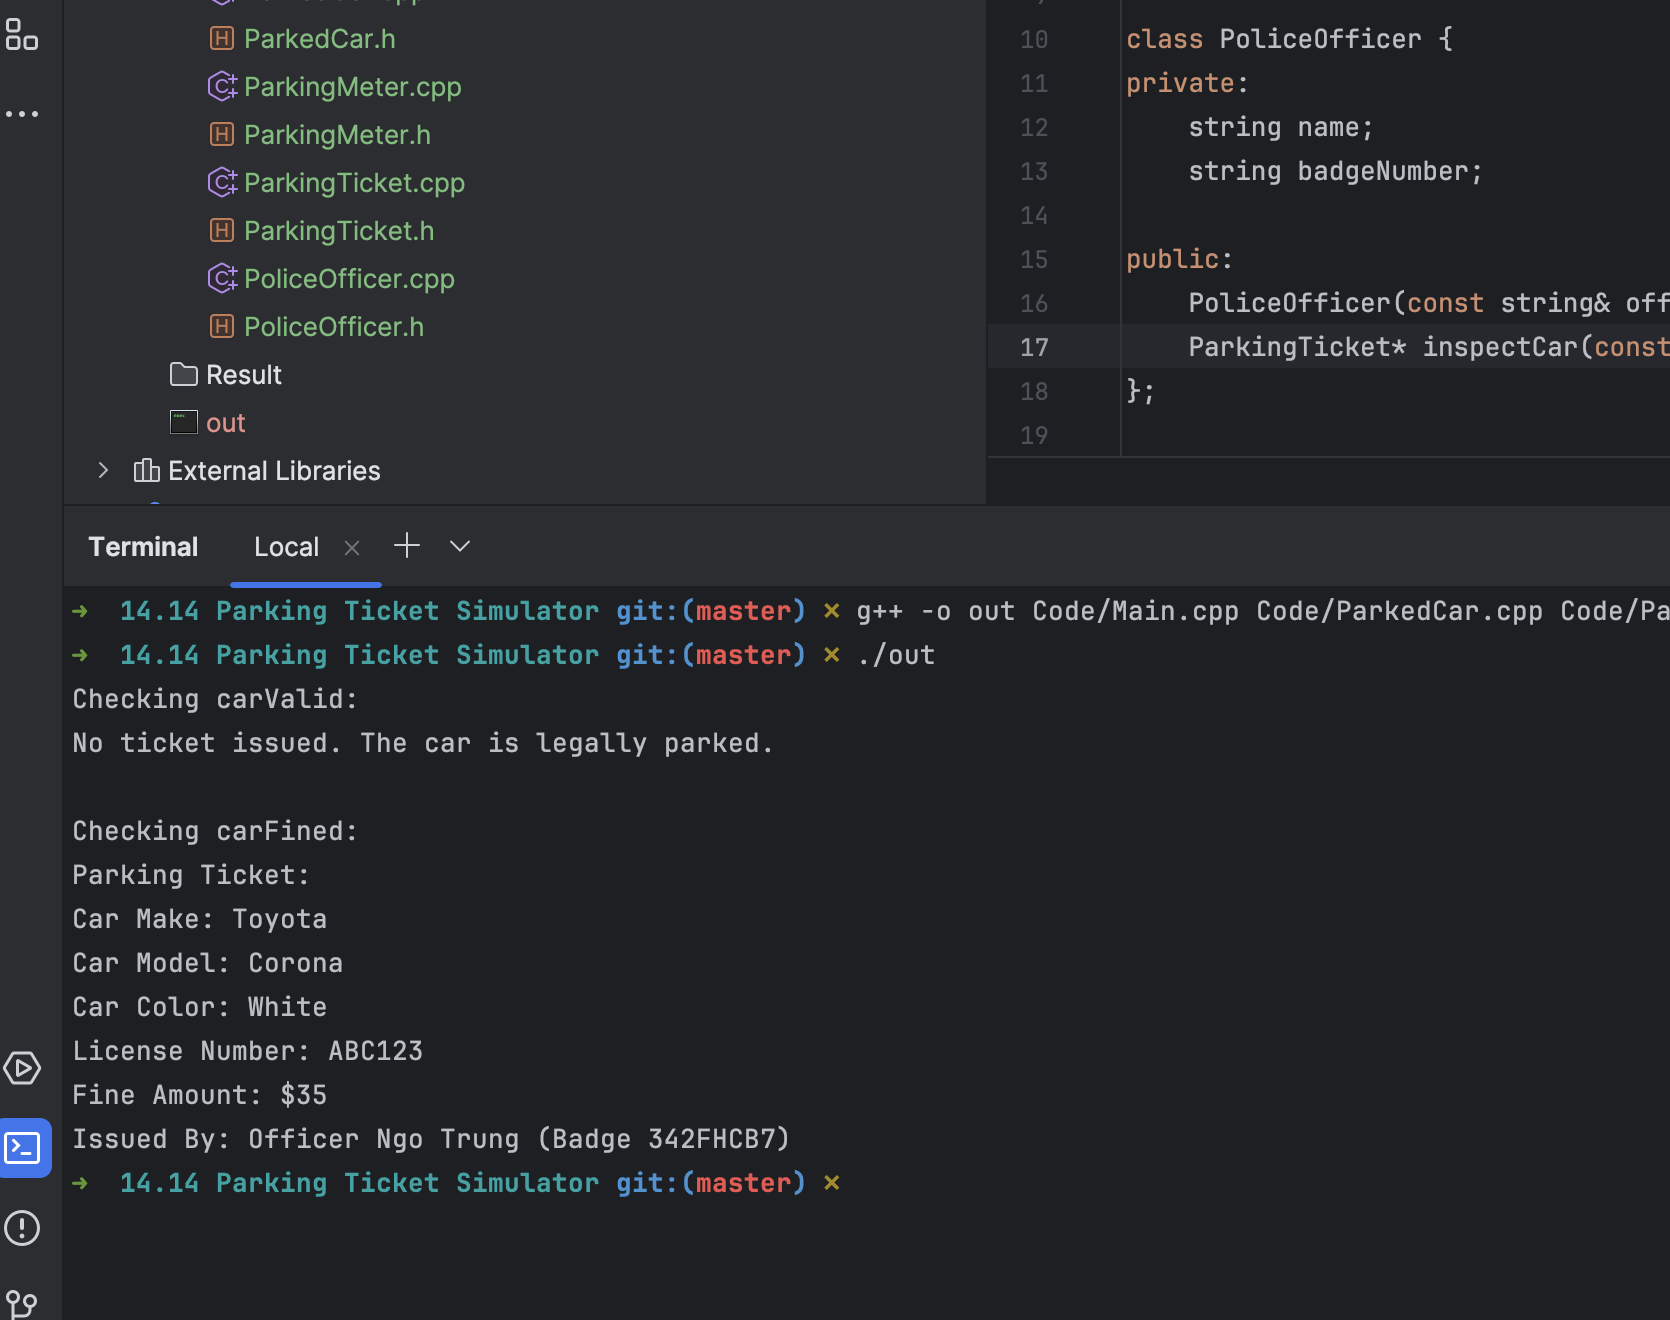
\includegraphics[width=0.8\textwidth]{./Assets/Results/Assignment12/4.png}
    \caption{14.14 Result}
\end{figure}
\end{document}

